\section{Traffic Scheduling} \label{sec:te}
\label{sec:scheduling}
% 根据需求说明一下 我们为什么需要进行流量调度,流量调度的输入从哪里来(性能数据 流的数据)(对应探测章节);如何建模进行域间流量的调度 以及对应的目标(对应4.1);控制器在接受到变化的路由表的时候,如何通过变化的路由将对应的流从出口a切换到出口b的(策略对应的粒度如何映射到的五元组最后将流进行切换)(对应4.2);
% 阐述调度的 系统 需求(目标)


% \textcolor{red}{The current scheduling scenarios independently perform optimal routing calculations based on business objectives, and ultimately detect and merge routing conflicts between scenarios at the routing layer. Analogous to the priority of different routing protocols on routers, the controller routing management module takes effect based on the priority of the scheduling type. The routing of high priority scheduling tasks takes effect, while the routing of low priority scheduling is suspended. It takes effect after the cancellation of high priority scheduling routes. The priority of scheduling tasks is: manual scheduling>fault scheduling>performance scheduling>cost scheduling>load balancing scheduling. This method effectively solves the conflict problem between different scheduling tasks, but due to the independent calculation of each scheduling task without considering the impact of other scheduling tasks, the calculated results are not globally optimal, and there is room for optimization and improvement.}

% {The goal of this research is to solve the optimal distribution solution of network traffic based on the Huawei cloud public network resource layout (PoP points + ISP operators + bandwidth), real-time traffic information, real-time performance dial test data, and network traffic cost unit price model, according to different network demands and corresponding priorities of business, and considering the impact of human operation and maintenance scheduling on traffic paths, And drive the underlying SDN traffic scheduling system for real-time traffic scheduling, achieving competitive performance and cost leadership while ensuring network stability and reliability.}

The aim of {\sys} is to address the optimal distribution solution for network traffic within the cloud public network resource layout. This involves considering the combination of PoP points, ISP operators, and bandwidth, along with real-time traffic information, performance dial test data, and a network traffic cost unit price model. By taking into account diverse network demands and corresponding business priorities, as well as the influence of human operation and maintenance scheduling on traffic paths, our objective is to drive the underlying SDN traffic scheduling system for real-time traffic scheduling. This approach enables us to achieve both competitive performance and cost leadership, while ensuring network stability and reliability.


\subsection{Problem Definition}
% Charging model;peering contract;% 以及和性能相关的协约规定 ,(相当于背景介绍)(不清楚放bg&motivation 还是这里)
% input output  % 要说明为什么只用出云不用入云带宽
In this section, we present a formalization of the task of cloud edge traffic engineering in a cloud network. 

Clients inherently prioritize aspects of their agreement with the cloud provider and may not be as concerned about aspects not explicitly specified in the agreement. 

Additionally, cloud providers are faced with the challenge of reducing inter-domain bandwidth costs in response to the rapid growth of traffic demand in cloud networks. 
Consequently, cloud providers focus on optimizing outbound traffic engineering to improve the performance of specific applications that cater to corresponding clients and minimize the overall cost of inter-domain bandwidth.

In our TE optimization, we have two objectives in terms of both performance-aware traffic and operation cost. 

Objective 1: Minimizing the total inter-domain $95^{th}$ percentile bandwidth cost. Our allocation scheme aims to determine a traffic assignment to ISP egress points over the entire billing period while minimizing the cumulative egress bandwidth cost. Typically, each ISP's cost is determined based on the $95^{th}$ percentile utilization of its resources.

Objective 2: Minimizing the weighted sum of performance factors in each time slot. The performance factors encompass variables such as latency, packet loss, and jitter, which collectively impact the quality of client experiences when accessing cloud content. We compute the weighted sum of these performance factors by aggregating the factors associated with all performance-sensitive flows, each weighted by its priority factor. The resulting weighted sum provides an aggregate measure of the overall performance experience for performance-sensitive clients during a specific time slot.




% {\sys} minimize bandwidth costs charged from ISP and backbone network billed by their utilization and minimize weighted latency of flows with high priority. We first introduce the following notation and formally specify the flow assignment problem: Given cost functions $Cost_{i}$ for each ISP  $i$, the flow assignment problem is to find allocation that minimizes the total cost $\sum_{i} c_{i}(p_{i}) + \sum_{g} c_{g}(\sum_{i} T_{ig})$. After the total cost is minimize, our framework further provides the flexibility to pick the operating point on cost-latency trade-off to minimize weighted latency of latency-sensitive flows $\sum_{f} L_{i}^{f}X_{i}^{f}P_{f})$ and finds allocations that best suit users need.

% \textbf{Objective function}. In our problem, we have two different objective: minimizes the total cost $\sum_{i} c_{i}(p_{i}) + \sum_{g} c_{g}(\sum_{i} T_{ig})$.  Let E = $\{e_{1}, e_{2}, ... , e_{n}\}$ be the set of all ISP from the WAN. Let a five-minute interval in the monthly billing period be $i$ where $i$ is in $\{1,2,..,M\}$. For instance, the month of January has $M$ = 8,928 five-minute intervals. The goal of our allocation scheme is to find a traffic assignment to ISP {\egresses} over the entire billing period such that the total bandwidth cost minimized. The cost incurred by each ISP is usually based on the 95th percentile utilization of that ISP, i.e., cost = $Cost(x)$, where $x$ is the charging volume and function $Cost(x)$ is the charging function. 

% The operator can decide for each destination prefix whether they want to: (i) optimize for the delay and/or loss; (ii) minimize the number of traffic shifts necessary to meet the requirements; or (iii) load-balance traffic by minimizing the difference between the most- and the least-used next-hop. Linear combinations of these or similar other objectives are easily implementable.

% \para{Constraint}
% Operational constraints: {\sys} admits constraints of two types: (i) those that limit the number of next-hops traffic can be spread on; and (ii) those that define performance constraints. Constraining the maximum number of next-hops per destination might be useful, for instance, to ease debugging. Performance constraints are maximum loss/delay values that traffic for a certain destination should experience. Defining such objectives is useful for meeting Service Level Agreements (SLAs) or particular application requirements

% Due to the uncertainty of the operator's network, network congestion or interruption often occurs, directly causing interruption or deterioration of user access to cloud services, leading to major network failures. To solve this problem, Cloud has built a self-developed network testing system, which uses its own probe to real-time test the network quality of a large number of end users. When there is an abnormality in the operator's network, based on network test data and its own network fault demarcation algorithm, it can quickly sense the faulty operator's line and precise province (or AS number), and drive the SDN scheduling platform to schedule the affected user network segments to the normal path, achieving rapid recovery from faults.

% Cloud overseas pop nodes usually connect with multiple operators, and users can access Cloud data center resources from their local AS. There are multiple paths that can reach them, but the latency quality of each path is inconsistent and they cannot choose their own path. Therefore, the current path may not be the optimal one. So if you want to achieve ultimate access performance, you need to conduct end-to-end quality detection on all accessible paths, and based on the detection results and routing principles, achieve the optimal end-to-end comprehensive quality path selection.

% An example: Taking a domestic operator as an example, in March, the traffic of the operator in the South China and North China regions exceeded that of the operator, while the traffic in East China exceeded that of the operator. By scheduling cloud traffic from East China to South and North China, BGP billing bandwidth can be reduced by 17G per month, saving costs of xxx million per month. 

% {\sys} minimize bandwidth costs charged from ISP and backbone network billed by their utilization and minimize weighted latency of flows with high priority. We first introduce the following notation and formally specify the flow assignment problem: Given cost functions $Cost_{i}$ for each ISP {\egress} $i$, the flow assignment problem is to find allocation that minimizes the total cost $\sum_{i} c_{i}(p_{i}) + \sum_{g} c_{g}(\sum_{i} T_{ig})$. After the total cost is minimize, our framework further provides the flexibility to pick the operating point on cost-latency trade-off to minimize weighted latency of latency-sensitive flows $\sum_{f} L_{i}^{f}X_{i}^{f}P_{f})$ and finds allocations that best suit users need.



% \textbf{Objective function}. 
% In our problem, we have two different objective: minimizes the total cost $\sum_{i} c_{i}(p_{i}) + \sum_{g} c_{g}(\sum_{i} T_{ig})$ and minimize
% Let E = $\{e_{1}, e_{2}, ... , e_{n}\}$ be the set of all ISP {\egresses} from the WAN. Let a five-minute interval in the monthly billing period be $i$ where $i$ is in $\{1,2,..,M\}$. For instance, the month of January has $M$ = 8,928 five-minute intervals. The goal of our allocation scheme is to find a traffic assignment to ISP {\egresses} over the entire billing period such that the total bandwidth cost minimized. The cost incurred by each ISP {\egress} is usually based on the 95th percentile utilization of that ISP, i.e., cost = $Cost(x)$, where $x$ is the charging volume and function $Cost(x)$ is the charging function. 

% \textbf{Constraints involved}. Our algorithm determine how much traffic should be allocated to each {\egress} in every time bucket over the whole billing period. The traffic allocations are subject to constraints on link capacities and backup reservation. For the offline problem, we assumes knowledge of traffic demands in the whole billing period, the traffic scheme must allocate flows to ISP {\egresses} in a way that the traffic demand is met in all time slots.



\subsection{Problem Decomposition}
Considering the two stated objectives, the first objective is focused on the minimization of the total inter-domain $95^{th}$ percentile bandwidth cost. It takes the overall bandwidth trends of the cloud as input and generates the final $95^{th}$ percentile billable bandwidth for each {\egress}. \textbf{Therefore, solving the $95^{th}$ percentile charging problem requires considering the entire time period and the bandwidth profile, without being sensitive to the specific flow scheduling per time slot.} The second objective, minimizing the weighted sum of performance factors, focuses solely on the actions of each performance-sensitive flow within each time slot, without considering the scheduling of other time slots or bandwidth trends. As a result, scheduling can be divided into two phases:

% \subsection{Offline Solution: Formulate Optimization Problem}


\begin{itemize}
\item
Phase I: Overall optimization (\S{\ref{sec:overall-opt}}), schedules bandwidth and optimizes the $95^{th}$ percentile outbound costs. It can be triggered actively or passively. Active triggering means running overall optimization periodically, such as monthly. Passive triggering means that overall optimization is triggered by a specific event, such as a significant fluctuation in the total bandwidth trend over the past three months. The goal of overall optimization is to ensure that the billable bandwidth for each {\egress} is as close to the true value as possible.

\item 
Phase II: Time slot optimization (\S{\ref{sec:timeslot-opt}}), which schedules flows and optimizes performance. Phase II is performed every time slot, as it needs to dynamically deal with the demand from the WAN in time for each time slot and output traffic allocation and flow assignment.

\end{itemize}

% 阐述一下p95问题(就这儿写收费模型,和Pretium那个论文的写法一样)一点背景 实际上是在分配带宽 且是一个np -hard 问题 以及 基于性能进行路由 是一个flow assignment problem, input output 是什么 
\renewcommand{\arraystretch}{1} % 增加行高
% \setlength\cellspacetoplimit{4pt}
% \setlength\cellspacebottomlimit{4pt}
\begin{table}
\centering
\begin{tabularx}{0.475\textwidth} { 
   >{\hsize=0.12\hsize\centering\arraybackslash}X 
  | >{\hsize=0.88\hsize\raggedright\arraybackslash}X }
 \hline
Symbol & Meaning \\\hline \hline
$E$ & Set of backbone links \\\hline
% $F_j$ & Set of all flows in time slot $j$\\\hline
$V$ & Set of PoPs \\\hline
$J$ & Set of time slots \\\hline
$L$ & Set of {\egresses} \\\hline
$m$ & Number of {\egresses} \\\hline
$n$ & Number of five-minute time slots in a month \\\hline
$l_i$ &  {\Egress} i \\\hline
$C_i$ & Capacity of {\egress} $l_i$  \\\hline
$C_{(u,v)}$ & Capacity of backbone link from PoP $u$ to PoP $v$  \\\hline
$L_u$ & Set of {\egress} of PoP $u$ \\\hline
$ub_i$ & Minimal billable bandwidth of {\egress} $l_i$\\\hline
$E_u^S$ & Set of outgoing backbone links from PoP $u$  \\\hline
$E_u^D$ & Set of incoming backbone links to PoP $u$  \\\hline
$c_i$ &  Peering rate (USD/Gbps) for {\egress} $l_i$ \\\hline
% $b^j_u$ & Default bandwidth of PoP $u$ in time slot $j$. It refers to the bandwidth of PoP $u$ before scheduling considering all flows egressing via their respective default {\egress} . \\\hline
% $b^j_{(u,v)}$ & Bandwidth of backbone link from PoP $u$ to PoP $v$ in time slot $j$\\\hline
% $p_i^j$ & Estimated 95th-percentile billable bandwidth of {\egress} $i$\\\hline
% $k_{i}^j$ & Whether {\egress} $i$ bursts in time slot $j$  \\\hline
% $y_i^j$ & Maximal available bandwidth of {\egress} $i$ in time slot $j$  \\\hline
% $x_i^f$ & Whether flow $f$ egresses via {\egress} $i$  \\\hline
% $x^f_{(u,v)}$ & Whether flow $f$ go through backbone link $(u,v)$ \\\hline
\end{tabularx}
\caption{\label{tab:common input}Common input parameters. Both the overall optimization phase and the time slot optimization phase will incorporate these parameters as input.}
\end{table}

\subsection{Overall Formulation}    \label{sec:overall-opt}
{In this section we formalize the task of overall optimization, which entails the minimization of interdomain bandwidth costs within a cloud network. Previous work \cite{goldenberg2004optimizing} has shown that the problem of optimizing costs under a percentile-based charging model is NP-Hard. We can transform the problem and formulate the traffic cost optimization problem as a Mixed Integer Linear Program (MILP), as shown in Algorithm \ref{alg1}. We implement the formulation using the OR-Tools solver \cite{or-tools}. Typically, as outbound traffic to paid peers is significantly higher than inbound \cite{singh2021costCascara}, we focus on minimizing the overall inter-domain bandwidth cost.}

% We denote $L=\{l_1, l_2,...,l_{\left| L \right|} \}$ as the set of all {\egresses}, where $\left| L \right|$ is the number of {\egresses}. And 
We define $p_i$ as the estimated billable bandwidth of egress $l_i$. The $p_i$ is the $95^{th}$ percentile bandwidth utilization of egress $l_i$ at the end of the billing period all of which minimizes the total bandwidth cost.
The core of the problem lies in how to determine the values of $\{p_1, p_2,..., p_{m}$, which should be able to minimize the total outbound bandwidth cost.

%The cost function consisting of the sum of 95th percentile utilization of links is non-convex. 
% We formalize the offline version of the problem of optimizing bandwidth costs for DCs. Previous work has shown that the problem of optimizing costs under percentile-based charging model is NP-Hard. However, based on insights described above, with the upper and lower bounds of $\sum_{i} p_{i}$, we can transform the problem and formulates the traffic cost optimization problem as a Mixed Integer Linear Program(MILP), as shown in Algorithm \ref{alg1}. We implement the formulation using the CSlover framework and solve it with the commercial optimization solver.

\para{Input parameters.}
The common input in Table \ref{tab:common input} comprises elements related to network topology, including both WAN infrastructure and cloud edge components. The cost of a {\egress} is determined by both the {\egress}'s peering rate and the billable bandwidth, where each {\egress}'s peering rate is determined and given by the peering ISP.

The $ub_i$ signifies that, regardless of whether the cloud uses {\egress} $l_i$ during the current billing period (usually one month), once the cloud procures {\egress} $l_i$, it incurs a minimum cost of $ub_i \cdot c_i$ for ISP peering. 

In addition to the common input parameters, we input the bandwidth demand of each PoPs $\{b^1_u, b^2_u, ..., b^n_u\}$ of one month and the corresponding total bandwidth demand $\{d_1, d_2,..., d_{n}\}$ of each slot in this month, which are predicted based on the previous three months' bandwidth data. 

 
A month consisting of 30 days has 8640 time slots.

\para{Decision variables.}
The overall optimization scheme assigns network flow to {\egress} in $L$, for every time slot $j$, $j\in[1,..,n]$. Let $p_i$ be the decision variable which refers to the estimated $95^{th}$ percentile billable bandwidth of {\egress} $l_i$. {\Egress} bursting is the allocation of the maximum available bandwidth to an {\egress}, with the precondition of avoiding congestion. Specifically, when $k_{i}^j$ is equal to 1, the bandwidth allocation of egress $l_i$ can be extended to $C_i$, and we refer to this as bursting. When $k_{i}^j$ is equal to 0, the bandwidth allocation of egress $l_i$ can only be extended to $p_i$, and we refer to this as not bursting.

% 如果 k 为 1 ,我们称之为 burst  % 因为我们是使用的预测数据输入的,因此 p_i 成为 estimated billable bandwidth


\para{Objective function.}
The objective of algorithm \ref{alg1} is to minimize the total outbound bandwidth cost incurred across all {\egresses}:
$$\min\sum_{l_i \in L} c_i p_i$$


\para{Constraints.}
As described in the background, the $95^{th}$ percentile billing model calculates the bandwidth cost while ignoring the top 5\% of bandwidth usage. This implies that 5\% of the total time slots are considered free or unused. During these free time slots, we can allocate maximum bandwidth to the {\egress}. Therefore, the number of times that an {\egress} can burst is constrained to 5\% of the total number of time slots. In addition, traffic allocations on an {\egress} are subject to the constraint of {\egress}'s capacity. For each {\egress} $l_i$, the traffic size of 5\% of the time slots is greater than or equal to $p_i$, and the traffic size of the remaining 95\% of the time slots is less than or equal to $p_i$. Most notably, traffic scheduling between different PoPs is subject to the constraint of backbone link capacity of backbone.

% {The first constraint states that 5\% of the total time slots in a month should be reserved for {\egress} bursting. The second constraint ensures that the total bandwidth demand during a specific time slot doesn't exceed the combined capacity of all {\egress}s. The third constraint specifies that the estimated chargeable bandwidth of {\egress}s should be greater than the guaranteed bandwidth. Furthermore, the fourth constraint dictates that the remaining bandwidth at the PoP - accounting for both incoming and outgoing bandwidth - must be less than or equal to the total available capacities of {\egress}s at the PoP. Additionally, the fifth constraint establishes that the bandwidth along the backbone link must be within its capacity constraint. Lastly, the sixth constraint mandates that there should be surplus bandwidth after scheduling within the PoP.}

% Cutting-edge optimization solvers use a combination of techniques to solve general Mixed Integer Programs (MIPs). At a high level, the first step is relaxing the MIP to an efficiently solvable Linear Program (LP) by removing the integral constraints. If a feasible solution to the LP is not found, the MIP, in turn, is also infeasible. If a feasible solution is found, the solution of the LP is a lower bound to the solution of the original MIP. Therefore, the LP solution provides the lower bound on bandwidth cost without having to solve the MILP. We note that Algorithm \ref{alg1} has O(mn) variables. Predicting the difficulty of Integer programs in terms of the number of variables and constraints is hard. Indeed, using upper bounds and lower bounds can efficiently reduce the solution space, which greatly reduces the algorithm’s running time. The reason behind this behavior is that only consider value between upper bounds and lower bounds make it easier for the optimization to find results which meet demands without violating constraints. Once the LP relaxation has been solved, MIP solvers find feasible solutions of the MIP problem from an exponential number of possibilities. 

% 是不是需要把这个表格里面的值 和 一个出口上的带宽进行一个比较?
\begin{table}[t]
\centering
\begin{tabularx} {0.480\textwidth} {|X|X|X|X|X|X|X|X|X|}
 \hline
PoP & JNB & StG & StP & MC & JKT & SP & HK & BKK \\\hline
JNB & 0 & 0.8 & 2 & 2 & 2 & 5 & 2 & 2 \\\hline
StG & 0.8 & 0 & 1.6 & 0.8 & 0.8 & 0.8 & 0.8 & 0.8 \\\hline
StP & 2 & 1.6 & 0 & 4 & 2.4 & 6 & 2.4 & 2.4 \\\hline
MC & 2 & 0.8 & 4 & 0 & 6 & 6 & 15 & 4 \\\hline
JKT & 2 & 0.8 & 2.4 & 6 & 0 & 40 & 16 & 4 \\\hline
SP & 5 & 0.8 & 6 & 6 & 40 & 0 & 200 & 10 \\\hline
HK & 2 & 0.8 & 2.4 & 15 & 16 & 200 & 0 & 10 \\\hline
BKK & 2 & 0.8 & 2.4 & 4 & 4 & 10 & 10 & 0 \\\hline
\end{tabularx}
\caption{\label{tab:backbone-lack} Lack of backbone capacity. The capacity variation among certain PoPs can indicate significant disparities in backbone capacity. Many of the backbone links suffer from insufficient capacity.}
\end{table}
% 搞成一个 heatmap吧

\para{Key insights.}
{To minimize the overall cost, we draw insights from the status quo of the operator's network and from our analysis of managing the 95th percentile outbound bandwidth cost:}
\begin{itemize}
\item{\para{Consideration of backbone link capacity insufficiency.} The assumption made in \cite{singh2021costCascara} presupposes that there is sufficient capacity between network nodes. empirical investigations conducted by network operators (\ref{tab:backbone-lack}), reveal that the capacity of backbone links between PoPs is considerably limited compared to the default bandwidth available of PoPs and {\egresses}. At the beginning of our experiment, we did not account for the impact of backbone capacity. We scheduled the bandwidth in a manner analogous to the conventional $95^{th}$ percentile method. However, we found that the limited backbone capacity made it difficult for the bandwidth to converge at a PoP where some {\egresses} were planned to burst. This resulted in the planned bursting {\egresses} being unable to burst, wasting 5\% of the free time slots and potentially increasing the billable bandwidth of {\egresses}. The experiment shows that the total cost of outbound bandwidth is even worse than the baseline, which does not switch the traffic and keeps it intact. To address this issue, we introduce the default bandwidth of each PoP into our formulation. This allows us to consider which backbone can be allocated more bandwidth and which should be allocated less. We achieve a ratio of outbound bandwidth cost optimization of approximately 36\%. This result confirms that the limited capacity between PoPs inevitably impacts the bandwidth scheduling for {\egresses}}.


\item
{\para{Principles of minimizing $95^{th}$ percentile bandwidth cost.} First, utilizing 5\% free time slots for each {\egress} (Figure \ref{fig:use-free-timeslots}). Each {\egress} bursting in the highest 5\% of its time slots does not increase its billable bandwidth. Therefore, each egress has 5\% of free time slots. These time slots should be fully utilized as much as possible for each link, and traffic should be shared through staggering peaks, which can reduce overall costs. 
Second, efficiently using the available capacity of {\egress} (Figure \ref{fig:use-95-timeslots}). During the 95\% of the time slots when an {\egress} does not burst, the total outbound bandwidth cost remains unchanged since the traffic volume is below the billable bandwidth threshold. Consequently, maximizing the utilization of available capacity below the billable bandwidth for this {\egress} during non-burst time slots can effectively alleviate the load on other {\egresses}, resulting in reduced overall costs.}
\end{itemize}

\iffalse
\begin{figure}
    \centering
    \subfigure[Utilizing 5\% free time slots for each {\egress}]{
    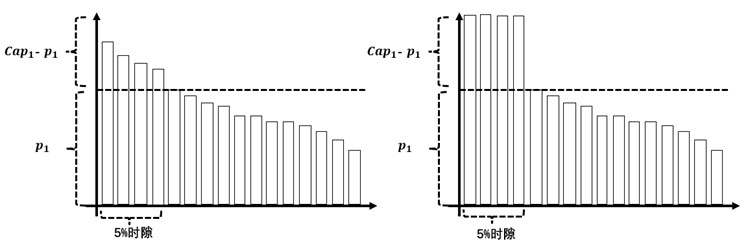
\includegraphics[width=8cm]{figs/implement/use-free-timeslots.jpg}}
    \vspace{0.5cm}
    \subfigure[Efficiently using the available capacity of {\egress}]{
    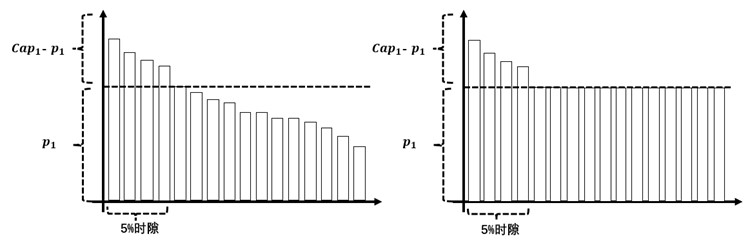
\includegraphics[width=8cm]{figs/implement/use-95-timeslots.jpg}}
    \caption{Bandwidth distribution of different time slots before and post $95^{th}$ percentile charging bandwidth optimization for a particular {\egress}}
    \label{fig:95-principles}
\end{figure}
\fi

\begin{figure}
    \centering
    \subfigure[Before optimization]{\label{fig:use-free-timeslots}
    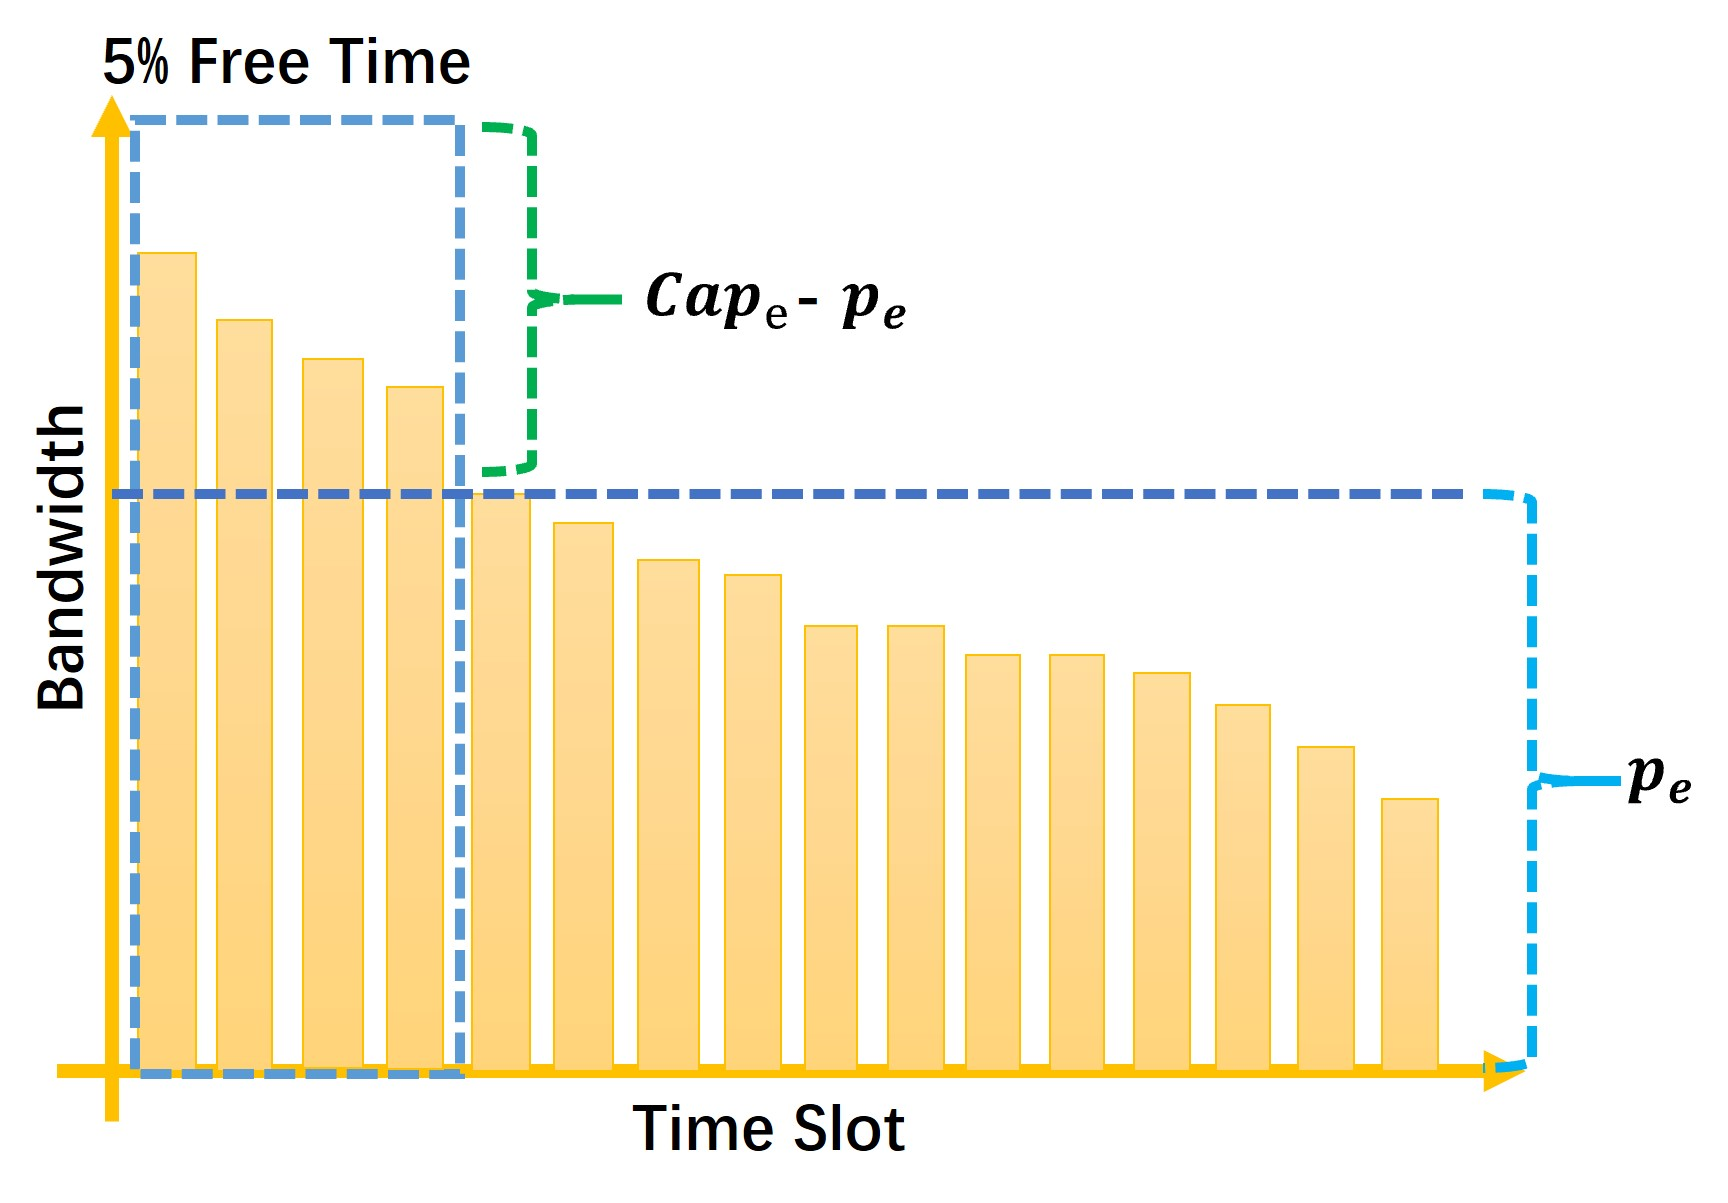
\includegraphics[width=3.9cm]{figs/implement/overallBeforeOpt.jpg}}
    \quad
    \subfigure[After optimization]{\label{fig:use-95-timeslots}
    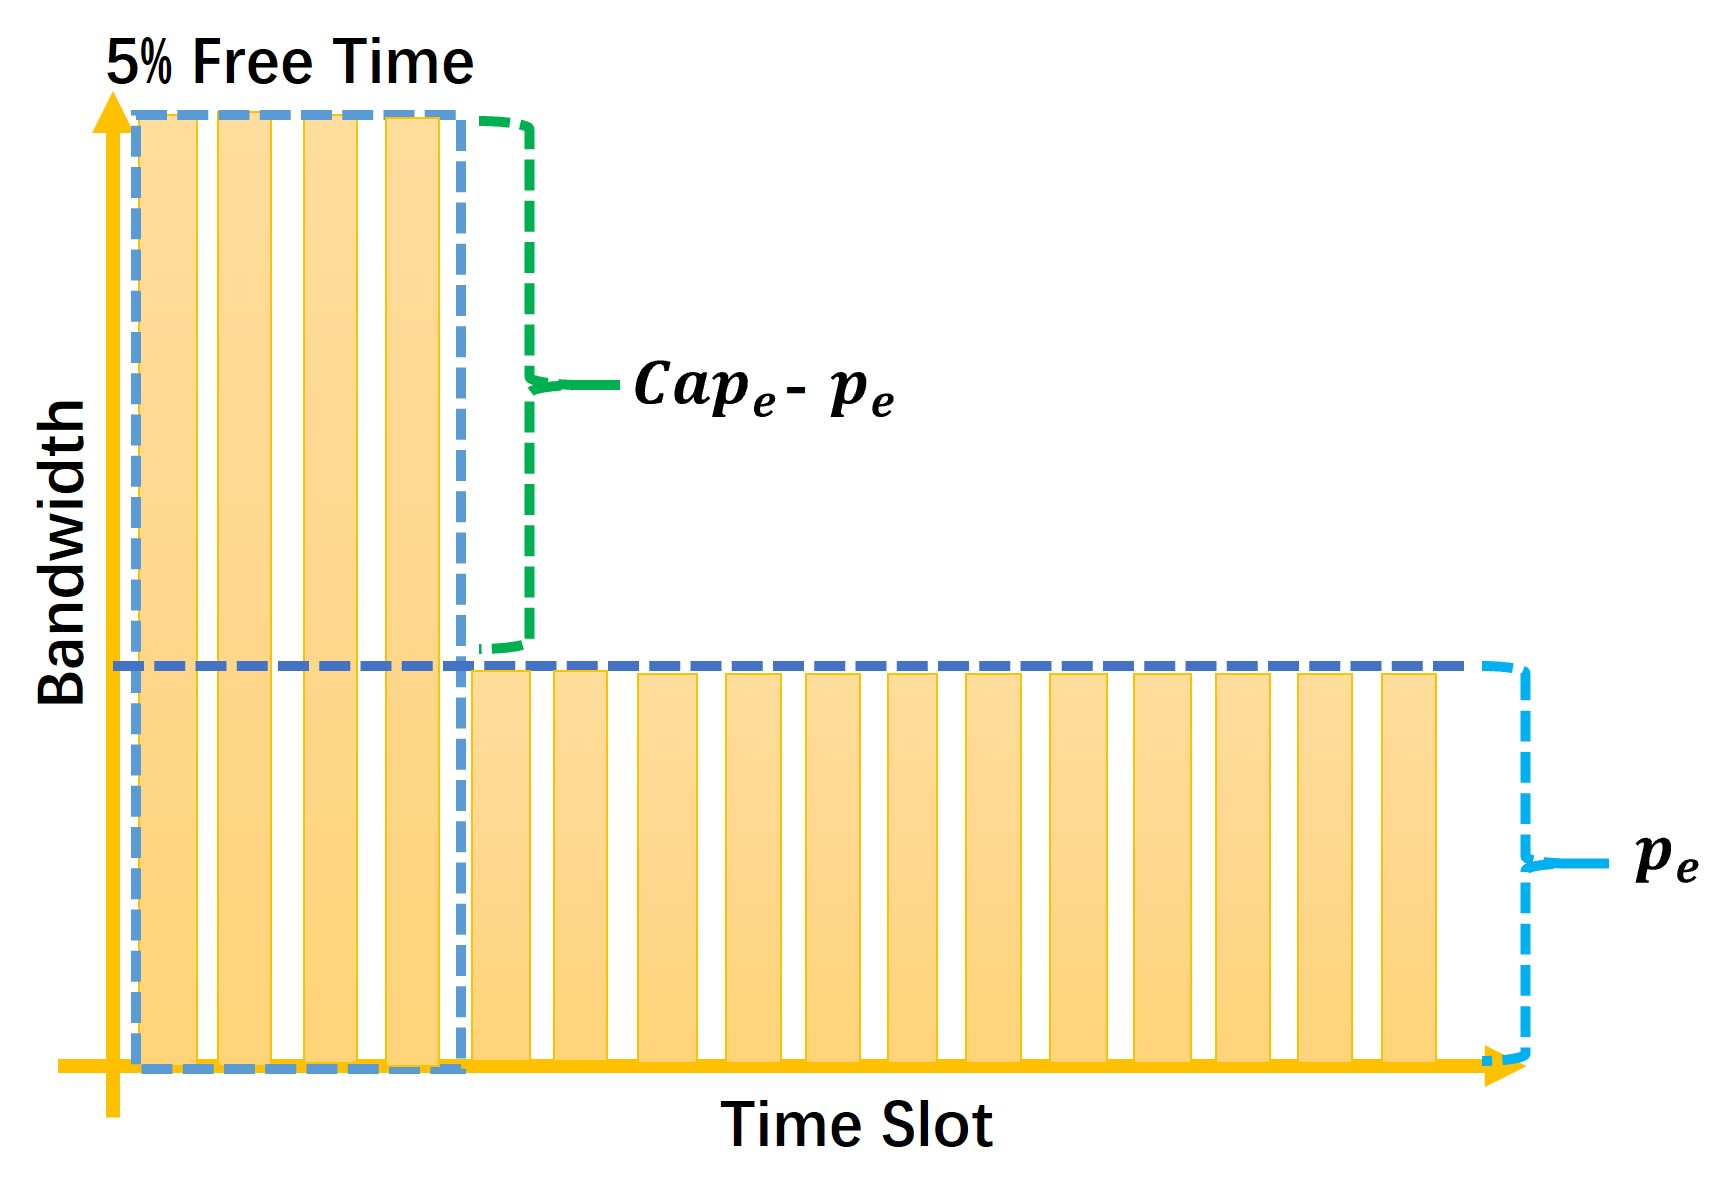
\includegraphics[width=3.9cm]{figs/implement/overallPostOpt.jpg}}
    \caption{Bandwidth distribution of different time slots before and post $95^{th}$ percentile charging bandwidth optimization for a specific {\egress}}
    \label{fig:95-problem2}
\end{figure}



% {Based on the definition of $p_i$ and the associated constraints, we can find a series of ways to determine the upper and lower bounds of $\sum_ip_i$. With the upper and lower bounds of $\sum_ip_i$, the algorithm starts from the lower bound of $\sum_ip_i$, and uses linear programming in a sequential traversal fashion for each value of $\sum_ip_i$ to compute the specific each $p_i$ and determine whether it is feasible or not. Feasible means that starting from this $\sum_ip_i$ value, a set of $p_1 p_2 p_3...p_n$ can be obtained without violating its own definition and the constraints of the associated backbone network links and egress.}


% {Thus, based on the definition of $p_i$ and the associated constraints, we can determine the upper and lower bounds of $\sum_ip_i$, which reduces the cost of the search. Then based on the fact that the total bandwidth of each time slot must be less than the total available capacity of the {\egress}s in the current time slot (the available capacity of the {\egress} $l_i$ for burst is $C_i$ and $p_i$ for non-burst). This is used to construct a mixed-integer plan with quadratic constraints, which is solved using the OR Tools solver.}



% {In addition, a series of optimizations are performed to improve the solution speed of the model:}

% {We find that $\sum_ip_i$ is currently continuous, and we can reduce the search space of the problem by discretizing $\sum_ip_i$. Also, the larger the value of $\sum_ip_i$, the more likely it is that the model will be able to solve a feasible solution, so we traversed the domain of the just-discretized $\sum_ip_i$ by bisecting it, which drastically reduced the number of search points. In the end, we are able to solve the problem in about 10 minutes or less. In addition, since our discretisation granularity is 1, the $95^{th}$ percentile utilization prediction for each {\egress} is within 1 of the theoretical optimum.}

% {Additionally, we have compressed the time slots for the solution, and we have compressed the number of time slots from more than 8,000 time slots in a month to 288 time slots. This is because the $95^{th}$ percentile utilization prediction results of each {\egress} are most relevant to the trend of total bandwidth and are not sensitive to the specific number of time slots. The daily bandwidth trend of Huawei Cloud is basically stable over a month, and the trend is basically the same after the 8000 time slots in a month are sorted in descending order according to the traffic size and the 288 time slots in a day are sorted in descending order according to the traffic size. Moreover, the overall level is somewhat tolerant to the accuracy, and since the real traffic trend and the actual bandwidth trend are bound to be different, the time slot level will fine-tune some unreasonable $p_i$ accordingly, so we  carry out such a compression.}


\para{Complexity Analysis}
% 总体层面挑战:求解器不可能在1H内完成千万级规模混合整数规划模型的求解
% 时隙数量:8640
% 变量数量:1500w+ 
% 约束数量:3000w+
Algorithm 1 considers the traffic generated within each PoP and the capacity constraints of the egress and backbone networks for all time slots in a month. Where the number of constraints reaches roughly O(n(|J|+|L|+|V|))
We provide the corresponding solution in Section \ref{sec:overall-slu}.

\subsection{Time Slot Formulation}  \label{sec:timeslot-opt}

The task of time slot optimization is to perform real-time flow scheduling in each time slot. Algorithm \ref{alg3} offers a formal description of the optimization problem. As we have done overall optimization scheduling the bandwidth across {\egresses}, time slot optimization is required to put specific flows onto the {\egresses} subject to the capacity constraints calculated by phase I. It is well-established that assigning flows to specific {\egresses} can be considered a generalized assignment problem (GAP) \cite{shmoys1993approximationGAP}, which has been proved an NP-hard combinatorial optimization problem and is typically solved as a MILP.

This optimization aims to enhance the performance of performance-sensitive flows and simultaneously manage outbound costs at a lower level. 
% 我们通过将流在 可用空间之下进行指派 从而保证出云成本的低水平
% 算法的位置,ref 要改成后面的简略版本

\para{Input parameters.}
{In addition to the common input parameters about the WAN and the edge of the cloud. The data input is all related to the current time slot $t$, including $b^t_{u}$ and $F^t$. $b^t_{u}$ denoting Default bandwidth of PoP $u$ in time slot $j$ refers to the bandwidth of PoP $u$ before scheduling considering all flows egressing via their respective default {\egress}. We need $b^t_{u}$ when dealing with constraints about backbone capacity. $F^t=\{f^t\}$ denotes all the demand flows from the WAN in time slot $t$. $y^t_i$ is the maximal available bandwidth in time slot $t$ described in phase I input parameters.}


\para{Decision variables.} The time slot optimization scheme assigns network flow to {\egresses} in $L$ in time slot $t$, $t\in[1,..,n]$. We introduce the decision variable $b^t_{(u,v)}$ to represent the bandwidth allocation on backbone link $(u,v)$ from PoP $u$ to PoP $v$ in time slot $t$. The binary decision variable $x_{(u,v)}^{f^{t}}$ indicates whether flow $f$ egresses through {\egress} $l_i$ within time slot $t$, and the binary decision variable $x_i^{f^{t}}$ indicates whether it traverses backbone link $(u,v)$ within time slot $t$.




\para{Objective function.}
The goal of our time slot optimization scheme is to find a flow assignment to edge links in the current time slot $t$ such that the current inter-domain bandwidth cost, the current weighted sum of the performance factor of all flows, and the remaining capacity of burst {\egress} is minimized. The cost in time slot $t$ incurred on {\egress} $l_i$ is the product of the peering rate ($c_i$) and the $95^{th}$ percentile utilization of that link (denoted by $p_i^t$). 

$$\min\sum_{l_i \in L} c_i \cdot p_i^t+\sum_{f^t \in F_s} w_1\left(V_f\right) x_i^{f^t}          \cdot perf(i, f^t) +w_2 \sum_{l_i \in L} y_i $$

\para{Constraints.} The constraints introduced in our formalization pertain to {\egresses}, backbones, and PoPs. The bandwidth allocation of a PoP depends on its outgoing, incoming, and default bandwidth. The assignment of a flow during time slot $t$ depends on the available capacity of {\egresses} and backbones.



% The constraints hold significant importance in the following order: Firstly, ensuring that the $95^{th}$ percentile bandwidth of each outlet in a time slot is not lower than the $95^{th}$ percentile bandwidth of the previous time slot. Secondly, each flow must select one of its available outlets, where $x_i^f$ can only be either 0 or 1. Thirdly, the total traffic carried by each outlet must not exceed its maximum available bandwidth. Fourthly, the traffic load on each backbone link should not exceed its maximum available bandwidth. Fifthly, each flow must traverse either an outlet within the source PoP or a backbone link. Sixthly, the number of incoming backbone links that each flow passes through within a non-source PoP should be equal to the number of incoming and outgoing flows. Seventhly, the flow rate of each PoP egress with a P4 device must be greater than or equal to 0 and should not exceed the sum of the available bandwidths of the egress links. Eighthly, the flow rate of each PoP without a P4 device through the backbone should be equal to the number of outgoing flows, indicating its transit role. Ninthly, the maximum available bandwidth of an egress with an exhaustive available punchdown slot equals the 95th percentile bandwidth. Finally, the maximum available bandwidth is set to the 95th percentile bandwidth. Additionally, there are constraints on the maximum available bandwidth of egresses for the available topping time slots: When $k_i=0$, the first two constraints are applied, introducing $y_i=k_i$. When $k_i=1$, the last two constraints are applied, introducing $y_i=C_i$.

\para{Key insights.}
% 根据总体层面计算出来的 pi 控制每个出口的分配带宽,从而使得流能够分配出去,同时还能控制出云总成本维持在一个低水平
% 冲顶问题综合考虑进时隙层面模型中,对比启发式地选择冲顶的出口。经过我们实际实验,如果启发式地选择小的出口进行冲顶,所选择的出口可能因为所在pop的 所有到达该pop的骨干网总容量过小,导致决策要冲顶的出口无法冲满,由此浪费了5%的冲顶空间。  % 后面的 时隙层面拆分了问题后的描述,可以说利用到了这个insight
{In the process of time slot optimization, we conducted a comprehensive analysis of prior research findings and examined negative experimental results. From this analysis, several valuable insights emerged:}
\begin{itemize}
\item \para{Assigning flows according to {\egress}'s billable bandwidth} The output of the flow assignment time slot optimization must adhere to the billable bandwidth constraints established during the overall optimization phase. It is crucial because the overall optimization strategy meticulously schedules bandwidth allocation to ensure that {\egresses} peak at the appropriate time slots, thereby minimizing outbound bandwidth costs.

\item \para{Deliberating the selection of bursting {\egresses}.}
As we discussed in the overall optimization, we incur the backbone constraints in computing each {\egress}'s estimated billable bandwidth. We adopt the heuristics akin to those found in \cite{singh2021costCascara,goldenberg2004optimizing} to select which {\egresses} is going to burst in the current time slot. However, the ratio of optimizing bandwidth cost was consistently approximately 4\%-7\% which confused us a lot. We found subsequently that the chosen {\egresses} may not be able to burst as we anticipate. The reason is that the limited incoming backbone capacity at the PoP results in poor incoming traffic, which cannot ensure the {\egresses} on the PoP burst up to a high bandwidth level. This must waste the number of 5\% free time slots to accommodate peak traffic. Thereby {\egresses} may encounter a shortage of available bursting time slots, necessitating an increase in billable bandwidth when facing peak traffic in the future. This, in turn, leads to elevated bandwidth costs. This drives us to formalize the selection of bursting {\egresses} and assignment of flows together. Notably, this insight motivates us to decompose the problem of time slot optimization into the subproblem of selecting bursting {\egresses} and heuristic to assign flows later \ref{Solving Optimization Quickly}. We achieve a ratio of outbound bandwidth cost optimization of approximately 36\% eventually, which reveals that deliberating the selection of bursting {\egresses} is much more important than we thought.

\end{itemize}

\para{Complexity Analysis.}
% 时隙层面挑战:求解器不可能在10s内完成亿级规模混合整数规划模型的求解
In Algorithm \ref{alg3}, constraints are imposed to ensure that the total flow bandwidth for each {\egress} and each backbone does not surpass the capacity limit. Consequently, the total number of constraints in Algorithm \ref{alg3} amounts to $O(|F|\dot (|E|+m))$, where $|F|$ represents the number of flows. In our testing topology, considering 2 million flows per time slot, Algorithm \ref{alg3} is projected to involve approximately 200 million constraints and 2 billion decision variables. {\sys} plans to conduct flow scheduling every five minutes, representing one time slot. This process encompasses actions such as data collection and command issuance. As a result, it's essential to maintain the algorithm's execution time at approximately 10 seconds per time slot. Although the linear programming solver can give an optimal solution, it is extremely slow and takes close to 1 minute just to schedule 10,000 flows. Therefore, the solver alone cannot meet our goal of scheduling 200 million flows per time slot. We provide the corresponding solution in Section \ref{sec:timeslot-slu} and Section \ref{sec:Network Slicing}.

%时隙数量:200w+
%变量数量:20亿+ 
%约束数量:2000w+



\section{Overall Optimization}\label{sec:overall-slu}
% 优化思路:通过对总流量排序后滑窗采样,降低模型规模,实现20min内求解
We have demonstrated the decomposition of our inter-domain TE optimization problem and the challeges in practice. In this section we discuss the solutions for the large-scale computation of routings.


\section{Timeslot Optimization}\label{sec:timeslot-slu}
% 要说一下 time slot 的那个形式化根本解不了
The main objective of the Timeslot Optimization is that we maintain the execution time of the algorithm in O(1) min. To this end, we introduce two optimization approachs. 

\begin{itemize}[leftmargin=*]  
\item \textbf{Optimization \#1: Only performance-aware flows and large flows are scheduled (\S\ref{Scale Characteristics}).} By observing the characteristics of the traffic distribution in the outgoing cloud, we find that we do not need to schedule all the flows and still achieve a sub-optimal objective. This optimization reduces the burden on the algorithm and also mitigates the problems of packet loss rate and increased latency caused by too much traffic scheduling. 
\item \textbf{Optimization \#2: Traffic is allocated to each PoP first then flows are scheduled. (\S\ref{Solving Optimization Quickly}).} We decompose the scheduling problem at the time slot level into a burst decision problem and a heuristic scheduling problem. The burst problem is still a linear programming problem, but its constraint variables are independent of the number of flows and are only related to the number of PoPs, the number of backbone links, and the number of {\egresses}, which has a good scalability. Flows are then scheduled by a heuristic method.
\end{itemize}

\subsection{Scale Characteristics} \label{Scale Characteristics}
% 问题规模分析 流量特征分析
% PoP, Edge Link, traffic. Or add a setting Section like paper Facebook Edge Fabric.
% Cloud networks occupy a central position in the Internet ecosystem due to the large volume and variety of popular content they serve to users. To make this possible, cloud providers  peer with a large number of networks or Autonomous Systems (ASes) on the Internet, including transit ISPs and eyeball networks.


We go over the distribution of the bandwidth of the different flows based on a week's worth of flow data collected for each time slot (from May 22, 2023 to May 28, 2023) for the {\egresses} on the existing network. As show in Figure \ref{fig:distriFlow}, that the flows utilizing 94.21\% of the total bandwidth comprise only 0.91\% of the overall flow count. In addition, we find that roughly 4.5\% of the total flows are performance-aware, accounting for approximately 0.8\% of the total bandwidth across all flows. 

\para{Key insights.} The final total cost is not related to the number of flows, but only to the bandwidth of the flows. From the characteristics of the flows, we find that a small number of large flows actually occupy the vast majority of the bandwidth. If only these large flows are scheduled, not only can the number of flows that need to be scheduled be drastically reduced, but at the same time the cost optimization is not significantly affected. Furthermore, given the relatively small proportion of performance-aware flows in the total flow count and our focus on performance optimization, we have included these flows in the scheduling process as well. In summary, we filter non-performance-aware small flows.

We designed a hyperparameter $FT$ to represent the filtering bandwidth threshold and we will discuss it in Section \ref{Evaluation}. Specifically, in the data collection phase, we will ignore all non-performance-aware flows with bandwidth less than $FT$. These flows will directly reach their current destination {\egresses}. After filtration with a proper $FT$ , the number of flows is reduced to about 1 per cent of its original size.

There are many benefits of filtering flows. Firstly, the system reduces the overhead of data collection, and the size of the flow data information that needs to be transmitted is reduced to about 1\% of its original size. Secondly, our algorithm reduces the time needed for scheduling. Faced with the size of 200 million flows, it is difficult to schedule all the flows within 10 seconds, even using heuristics. The reduction in the number of flows makes the algorithm runtime requirement possible. In addition, the reduction in the number of flows to be scheduled means that problems such as packet loss rate and increased latency caused by scheduling will be reduced. Choosing a proper hyperparameter $FT$ for filtering will not significantly reduce the effectiveness of the cost optimization, as we will show in Section \ref{Cost Optimization}.

% \begin{figure}
% 	\centering
% 	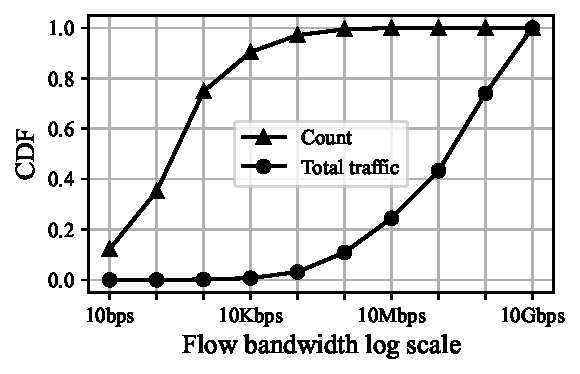
\includegraphics[width = 8cm]{figs/implement/bigflowdistribution.pdf}
% 	\caption{\small Distribution of flows by bandwidth}
% 	\label{fig:flowdistribution}
% \end{figure}

\begin{figure}
    \centering
    \subfigure[Distribution of flows by bandwidth]{
    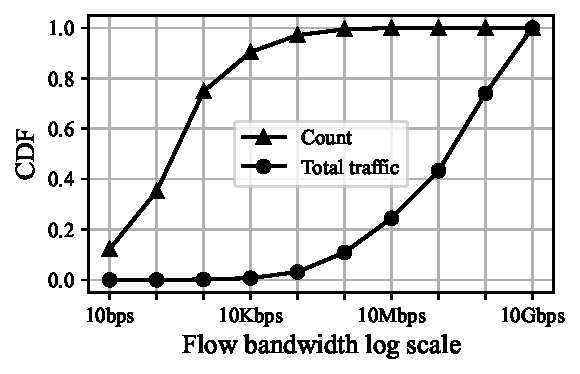
\includegraphics[width=3.9cm]{figs/implement/bigflowdistribution.pdf}}
    \label{fig:distriAllFlow}
    \quad
    \subfigure[Distribution of performance-aware flows by bandwidth]{
    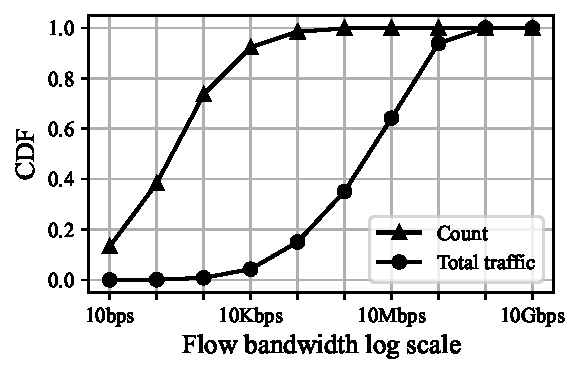
\includegraphics[width=3.9cm]{figs/implement/bigflowdistribution-2.pdf}}
    \caption{Bandwidth distribution of outgoing cloud traffic in a specific time slot}
    \label{fig:distriPerfFlow}
    \label{fig:distriFlow}
\end{figure}

% In order to be able to place more of the large flows into the more tightly constrained {\egresses}, while also taking into account the delay optimization of the delayed flows. We place the small performance-aware flows to the optimal {\egress} first using heuristics strategy and then consider the placement of the remain large flows.}

\subsection{Solving Optimization Quickly} \label{Solving Optimization Quickly}
% 是否应该把总体层面的加速 也放到这章?

In this section, we propose a time slot level problem decomposition method. The method decomposes the original linear programming problem into a new linear programming problem and a heuristic method, which greatly improves the scheduling efficiency. The new linear programming problem has better scalability because the decision variables are independent of the number of flows.

% The main challenges are:

% {For traffic scheduling at the time slot level, the scheduling algorithm needs to determine the {\egress} they should choose for each specific flow, which needs to take into account the objectives of backbone network constraints and flow delay and size. In addition, the algorithm design should consider performance issues to adapt to future large-scale traffic scheduling. The currently available data of the existing network shows that there are about 2 million flows (service + target prefix) in one time slot. There are still most of the {\egresses} in the existing network that do not have the ability to collect flow lists. If we consider the future upgrading of {\egress} equipment, all of which can collect flow list data, then it is estimated that there will be more than 100 million flows if the service size remains unchanged, so how to accelerate the problem solving becomes critical. Accelerated solving is mainly divided into: a) Reducing the number of variables. b) Cutting the original problem into sub-problems and solving them in parallel. In this subsection, we focus on reducing the number of flows involved in the original problem, i.e., reducing the number of decision variables $X_e^f$.}

\para{Key insights.} We integrate the considerations of algorithmic complexity at the time slot level with specific scenarios to summarize the following pivotal insights:

\begin{itemize}
\item \para{Schedule the traffic first and then schedule the specific flows.} The reason for the high complexity of Algorithm \ref{alg3} is that it schedules every flow. If it is assumed that each flow can be divided at any granularity according to the bandwidth, then the complexity of the algorithm at the time slot level is independent of the number of flows. Finally, we can do heuristic scheduling for the flows and transform the scheduling problem into a bin packing problem. This assumption is validated by the efficiency of the greedy algorithm for the bin packing problem, particularly when a significant portion of the items is of small size, enabling the algorithm to achieve high approximation ratios. As we mentioned in Section \ref{Scale Characteristics}, the characteristics of the flows exactly satisfy this property.
\item \para{Considering the capacity constraints of the backbone network in conjunction with the burst decision problem.} When all egresses within a Point of Presence (PoP) reach full capacity, the remaining flows must be directed to egresses in other PoPs. Determining the appropriate backbone for each flow and deciding which PoP to schedule it to presents a complex challenge. Directly applying heuristics to schedule flows might lead to instances where the backbone capacity is inadequate, resulting in these flows being unable to find a feasible {\egress}. Therefore, we opted to utilize an intermediate variable from the burst decision problem, specifically the used capacity of each backbone link, to guide the heuristic scheduling process.
\end{itemize}

% {We find that to utilize the $P_i$ of {\egresses} solved in the overall optimization, we have to fully utilize the limited backbone links. In addition, the selection of the burst {\egress} in each time slot is also a problem, both in terms of making the wastage of {\egress} bandwidth in each time slot as small as possible in order to save cost, and ensuring that after the selected {\egress} bursting, the flows in each PoP can be scheduled as much as possible and meet the capacity constraints of the backbone network. Therefore, we believe that the burst problem is closely related to the backbone capacity constraint problem. We design a method that gives the backbone physical link usage suggestions when making the burst decision, and meets the scalability at the same time, which means the complexity of the algorithm is independent of the number of flows. Specifically, we formalize the burst problem and the backbone limit uniformly, and the formalization is only related to the number of PoPs and the number of backbone links. After we solve this formalized problem using the solver, we are able to obtain not only the burst {\egresses} in each time slot, but also recommendations for the use of each physical link of the backbone network. Based on these recommendations, inter-PoP flow scheduling is performed to fully utilize the bandwidth of the backbone network.}

{In summary, the algorithm at the time slot level should be able to satisfy the performance needs and total cost of each {\egress} as low as possible after scheduling, while also considering the algorithm efficiency and scalability when the scale increases in the future. {\sys} time slot level algorithm takes these two problems into account and it can make parallel scheduling simple.}

% \subsubsection{Choosing burst links}

{\para{{\Egress} burst decision.} Due to the capacity constraints of the backbone network, the {\egress} burst decision problem is difficult to get an optimal solution using heuristics. In order to find an optimal and maintain good performance and scalability, the problem can be formalized as Algorithm \ref{alg4}}.

{On the one hand, the scheduling granularity is transformed into the bandwidth granularity. Therefore, the solver only needs to count the current sum of flow bandwidths in each PoP, independent of the number of flows, which ensures the high performance and scalability of the solver. On the other hand, the objective function ensures that the capacity wastage of all the {\egresses} is as low as possible, which can ensure that the burst capacity is fully utilized, which is conducive to reducing the final costs.}

% \subsubsection{From underlay to overlay}

{\para{Determining the virtual link bandwidth for inter-PoP scheduling.} We find that to effectively reduce the final cost, the capacity of the backbone network must be utilized. This is because the guaranteed bandwidth of the {\egress} of some PoPs is already sufficient to accommodate all the traffic within the PoP, while the traffic of some PoPs may be higher than the sum of the $p_i$ of the {\egress}s within the PoP. For this reason, we utilize the intermediate result of the burst decision problem in the first step: the usage of each backbone link. This result actually represents the amount of bandwidth per backbone that should be used by the solver in obtaining the optimal burst {\egress}, which we refer to as the recommended bandwidth of the physical links of the backbone. We want to use this result to guide how much bandwidth flows should be scheduled between PoPs. So the purpose of the second step is to get the recommended bandwidth of the virtual links between PoPs based on the recommended bandwidth of the physical links of the backbone network.}

{This problem can be modeled as the following: each PoP can be regarded as a vertex and the backbone network physical links can be regarded as edges. We use vertex $u$ to denote PoP $u$, edge $(u,v)$ to denote the backbone physical link from PoP $u$ to PoP $v$, $w_u$ to denote the total bandwidth of the current flow of PoP $u$, $w_{(u,v)}$ to denote the suggestion bandwidth of the backbone physical link from PoP $u$ to PoP $v$, and $G=(V, E)$ to denote the directed graph constructed by the above method. This algorithm can be described as the following steps:}

\begin{itemize}[leftmargin=*] 
\item[1] Confirm how much bandwidth each PoP needs to flow in/out. The bandwidth $O_u$ that $pop_u$ needs to flow out can be expressed as $O_u=\sum_{v\in V} |w_{(u,v)}-w_{(v,u)}| $. If the value is negative, it means that $pop_u$ requires inflow bandwidth.
\item[2] Sort $O_u$ from largest to smallest. That is, we should try to consider those PoPs with the largest outflow requirements first. Because we want to get as few virtual links as possible, and the scheduling of PoP-to-PoP flows is as centralized as possible.
\item[3] Consider the PoP with the largest $O_u$ each time, and bisect the largest flow that this PoP can schedule this time, denoted as $B$. After that, recursively start from point $u$ in the graph $G$, and each time choose an outgoing edge with the largest $w_{(u,v)}$ that is not smaller than $B$ until we find a point $p$ satisfying $-O_p\ge M$, which indicates that a flow of size $B$ can be scheduled from PoP $u$ to PoP $p$. Adjust the bisecting pointer to find the maximum feasible $B$. Then record the suggested bandwidth $F_{(u,p)}+=M$ for the virtual link from PoP $u$ to PoP $p$. And set $w_u-=M,w_p+=M$, and the edge weights of all edges on the path are subtracted from $B$.
\item[4] Keep doing step 3 until $w_u=0$ for any $u\in V$.
\end{itemize}

{Finally, the proposed bandwidth $F_{(u,v)}$ of the virtual link between PoP $u$ and PoP $v$ can be obtained. The algorithm in this step is also independent of the number of flows and has good scalability. The time complexity of the above algorithm is expected to be $O(|V|^2 |E| log(\max O_u))$, where $|V|$ is the number of PoPs and $|E|$ is the number of physical links in the backbone network.}

% \subsubsection{Heuristic assignment}

{\para{Heuristic scheduling.} Heuristic scheduling requires the use of the suggested bandwidth of the virtual link solved in the previous step. The principle is to make the actual used capacity of the virtual links equal to the recommended capacity as much as possible, so the algorithm needs to perform inter-PoP scheduling first. Since the number of performance-aware flows is small and the bandwidth is generally small, and the inter-PoP latency is high and the performance-aware flows tend to be scheduled within its orginal PoP, it is sufficient to schedule the performance-aware flows directly to the feasible {\egress} with the greatest performance (i.e. find the smallest {\egress} $l_i$ minimize the $perf$ function in Algorithm \ref{alg3}). The scheduling only needs to consider not exceeding the capacity limit of each {\egress} and not exceeding the recommended bandwidth limit of the inter-PoP virtual links.}

{Then the other non-performance-aware flows are scheduled, which can be regarded as a bin packing problem and the these flows need to be sorted from largest to smallest according to the bandwidth before scheduling, so that they can better fill up the {\egress} capacity and the suggested bandwidth of the virtual links as much as possible. Then, priority is given to ensure that links across the PoP are filled before scheduling flows within the PoP. After enumerating all the flows, there may be a remaining fraction of flows that cannot find a feasible {\egress}.}

{\para{Increasing $p_i$}. After heuristic scheduling, the total bandwidth of the remaining flows is often very small (typically less than 0.1Gbps in tests), so this step does not significantly increase the $p_i$ of a particular {\egress}. This step requires the remaining flows to be placed to a {\egress} that minimizes the cost of increasing the $p_i$ of the {\egress} after the flows have been placed to that {\egress}. The backbone physical link limitation problem can be considered by subtracting the recommended bandwidth given in the first step from the capacity of the backbone physical link, which is the available bandwidth at this time. When cross-PoP scheduling, determine whether the available bandwidth of the physical link between the two PoPs is greater than the bandwidth of the flow to determine whether the flow can be scheduled between the two PoPs.}



% Results of the offline allocation algorithm show that there is significant potential for optimizing bandwidth cost at the cloud edge. There are two caveats to the scheme’s use: first, it assumes knowledge of outbound demand for every time slot of the billing cycle. In practice, an online algorithm that can allocate network flows to peer links without the knowledge of future demands is required. Second, the optimization formulation takes 10 minutes on average to provide optimal traffic allocations for the entire month. However, state-of-the-art TE controllers compute traffic allocations every minutes, making it crucial to have an online solution that is efficient and effective. In this section we develop a heuristic-based online traffic allocation framework that uses insights from the offline optimal solutions and get results close to optimal.

% Despite the complexity of the cost optimization problem, we show that a simple and efficient algorithm enable the closeness of the heuristic solution to the offline optimal by using insights described before. The heuristic allocation achieves bandwidth costs savings within 10\% of the optimal.

% A key to optimizing cost is to determine the charging volumes for all ISP {\egresses}. For example, when ISPs use the 95th-percentile charging model, we need to determine the 95th-percentile traffic volume for each {\egress}. Once we know the charging volume for each ISP {\egress}, we can assign traffic by ensuring that the number of intervals in which each ISP $i$ serves more than its charging volume of traffic does not exceed 5\%. To make it clear, we introduce the definition of non-peak intervals and peak intervals. According to the definition of $\sum_{i} p_{i}$, during the intervals when total traffic volumes are no larger than $\sum_{i} p_{i}$, all traffic can be assigned without having any ISP receiving traffic more than its charging volume. Therefore, we call these intervals non-peak intervals. For the remaining intervals, at least one ISP needs to serve traffic more than its charging volume. As a result, we call the latter intervals peak intervals. We will use this terminology throughout this paper.
% Based on the above observation, we develop an efficient algorithm that computes an optimal traffic assignment in two steps: (i)compute the optimal charging volume for each ISP, and (ii) assign traffic based on the charging volumes computed.

% In this section, we first describe how to compute the optimal charging volumes to minimize total cost. We show that the optimal charging volumes for each ISP {\egress} can be derived in two steps: (i) compute the sum of the charging volumes, namely $\sum_{i} p_{i}$, and (ii) compute individual $p_{i}$ values based on $\sum_{i} p_{i}$ for each {\egress}.

% \subsubsection{Computing the Sum of Charging Volumes $\sum_{i} p_{i}$}
% We first describe how to compute the sum of charging volumes to minimize cost. Our observation is that the total cost has a monotonous property with respect to the sum of the charging volumes. This monotonous property suggests that to minimize the total cost $\sum_{i} Cost_{i}(p_{i})$, we need to minimize the value of $\sum_{i} p_{i}$.

% With the upper and lower bounds of $\sum_{i} p_{i}$, our algorithm starts from the lower bound of $\sum_{i} p_{i}$ and finds a feasible $\sum_{i} p_{i}$ value by traversing sequentially from the lower bound to the upper bound until it finds a feasible solution. Denote the upper bound of $\sum_{i} p_{i}$ as $Upper_{pe}$ and lower bound as $Lower_{pe}$. 
% We use the algorithm in Algorithm \ref{alg2} to figure out feasible value of $\sum_{i} p_{i}$ which is close to optimal. The basic idea is to properly choose the value of $\sum_{i} p_{i}$, so that multiple burst ISPs during each interval can together provide enough total capacity to carry all of the traffic demand in that time slot. More formally, given the corresponding traffic data and the set $\{p_{1}, p_{2}, ..., p_{i}\}$, we need to know IsPeAssignable(), i.e., whether it is possible to assign all ISPs {\egresses} to burst in peak intervals so that (i) no ISP $i$ bursts more than 5\% intervals, and (ii) there is enough total capacity in each interval to serve traffic demand. We want to find feasible solution which is close to optimal and meet the requirement described before with $f$ and the corresponding $\sum_{i} p_{i}$ as small as possible. The ways to check the feasibility and implement function IsPeAssignable() are multiple, like Heuristic solution from bin-covering problem or LP solution described in Appendix.

% \begin{algorithm}
% 	\caption{An online optimal flow assignment algorithm for
% 		splittable flows under the percentile-based charging model}
% 	\label{alg2}
% 	\begin{algorithmic}
% 		\STATE $P = Lower_{p_{i}}$
% 		\STATE $feasible$ = false	
% 		\WHILE {$feasible$ is false and $P \leq Upper_{p_{i}}$}
% 		\STATE $\sum_{i} p_{i} = \mathrm{qt}\left(V, P\right)$
% 		\STATE compute individual $p_{i}$ values 
% 		\STATE $feasible$ = IsAssignable()
% 		\STATE add $P$ by $\alpha$ if $feasible$ is false 
% 		\ENDWHILE
% 		\STATE Assign peak intervals such that each ISP $i$ bursts in at most 5\% intervals
% 	\end{algorithmic}
% \end{algorithm}




% \subsubsection{Computing Individual $p_{i}$ Values}
% Once $\sum_{i} p_{i}$ is determined, the next step is to compute the optimal charging volumes $p_{i}$ for each {\egress} $i$, which minimize $\sum_{i} Cost_{i}\left(p_{i}\right)$ subject to the computed $\sum_{i} p_{i}$. After each $p_{i}$ is computed, the set $\{p_{1}, p_{2}, ..., p_{i}\}$ helps to guide the detailed allocation of flows to each ISP {\egress} in every time intervals during the whole charging period. 
% We can figure out the optimal charging volume set $\{p_{1}, p_{2}, ..., p_{i}\}$ using dynamic programming algorithm or greedy algorithm, depended on the type of cost functions $Cost_{i}$.
% For simple cost functions like unit cost functions, where the user pays the ISP the product of an agreed-upon unit cost (in dollars per Mbps) and the billable traffic (in Mbps), greedy algorithm is enough to compute the optimal charging volume set $\{p_{1}, p_{2}, ..., p_{i}\}$ by assign the cheapest ISP {\egress} with the highest $p_{i}$ under its capacity constraints, which is easy to implement and provide the smallest cost.

% Since the real-world problem calls for online solution, we need to predict $\sum_{i} p_{i}$ in order to decide whether the next interval is a peak interval. Clearly, if we underestimate $\sum_{i} p_{i}$, then we may end up exhausting the quota of peak intervals too early, thus increasing the total cost due to increased charging volumes of individual ISPs. To avoid this penalty, we update $\sum_{i} p_{i}$ in the following conservative way. We use the $\sum_{i} p_{i}$ in the past charging period as an initial estimate of $\sum_{i} p_{i}$. We also maintain a sliding window (with length equal to the charging period) and after each interval we compute the $\sum_{i} p_{i}$ value for the most recent sliding window, denoted as $new \sum_{i} p_{i}$. Whenever $new \sum_{i} p_{i}$ exceeds $\sum_{i} p_{i}$, we increase $\sum_{i} p_{i}$ to $v * new \sum_{i} p_{i}$ and recompute all the charging volumes based on the new $\sum_{i} p_{i}$. For our traces, with $v = 1.05$ we are able to track increases in $\sum_{i} p_{i}$ quickly without overshooting too much.

% Given the charging volumes, namely $p_{i}$ for ISP $i$, next we describe how to assign traffic during each time interval. The goal of traffic assignment is to ensure that $p_{i}$ is the charging volume for ISP $i$; that is, for $q_{i} * I$ intervals, the traffic volumes assigned to ISP $i$ are less than or equal to $p_{i}$, and ISP $i$ is only allowed to serve more than $p_{i}$ for the remaining $\left(1-q_{i}\right) * I$ intervals. 

% This can be achieved by dividing intervals into non-peak intervals and peak intervals. Based on the definitions of peak and non-peak intervals, we assign traffic in the following way. If an interval is a non-peak interval, we assign traffic such that the traffic assigned to ISP $i$ is less than or equal to $p_{i}$. There are multiple ways to assign traffic to satisfy the above constraint. For a peak interval, we select an ISP $i$ to burst (i.e., its assigned traffic exceeds $p_{i}$). This is done by assigning each of the remaining ISPs its charging volume $p_{i}$, and then assigning all remaining traffic to the burst ISP. 


% \textcolor{blue}{For traffic scheduling at the time slot level, the scheduling algorithm needs to determine the egress they should choose for each specific flow, which needs to take into account the objectives of backbone network constraints and service flow delay and cost. In addition, the algorithm design should consider performance issues to adapt to future large-scale traffic scheduling. The currently available data of the existing network shows that there are about 2 million flows (service + target prefix) in one time slot. There are still most of the egress links in the existing network that do not have the ability to collect flow lists. If we consider the future upgrading of egress equipment, all of which can collect flow list data, then it is estimated that there will be more than 100 million flows if the service size remains unchanged, so how to accelerate the problem solving becomes critical. Accelerated solving is mainly divided into: a) Reducing the number of variables. b) Cutting the original problem into sub-problems and solving them in parallel. In this subsection, we focus on reducing the number of streams involved in the original problem, i.e., reducing the number of decision variables $X_e^f$ at the exit of stream assignment.}

% {We go over the probability distribution of the sizes of the different streams based on a week's worth of stream data collected for each time slot (May 22, 2023 to May 28, 2023) for the egresses on the existing network with P4 switches. We find that the streams that account for 94.21\% of the total bandwidth are only 0.91\% of the total number of streams in terms of number. An observation based on a deeper understanding of the 95 bandwidth optimization problem: the larger the bandwidth, the greater the impact that streams cause on cost regulation. Therefore, we can use only the large streams to participate in the solution of the original problem, and the remaining portion of the smaller streams are assigned to the links using heuristics. In order to be able to put more of the large flows into the more tightly constrained egresss, while also taking into account the delay optimization of the delayed flows. We put all the small cost streams into the default egress; assign the small delay streams to the egress first using heuristics; and then consider the assignment of the large cost streams.}

% {We find that to utilize the sum of egress $P_i$ solved at the aggregate level, we have to fully utilize the limited backbone links, so we need to design an algorithm to do this. In addition, the selection of the topping egress in each time slot is also a problem, both in terms of making the wastage of egress bandwidth in each time slot as small as possible in order to save cost, and on the other hand, ensuring that after the selected egress has been topped, the streams in each pop can be allocated as much as possible and meet the capacity constraints of the backbone network. Therefore, we believe that the topping problem is closely related to the backbone capacity constraint problem. Thus, we design a method that gives the backbone physical link usage when making the topping decision, and consider the scalability problem, which should not be too complex and the complexity should be as independent of the number of flows as possible. Specifically, we formalize the egress topping problem and the backbone limit uniformly, and the formalization is only related to the number of pops, the number of backbone links, and not the number of streams. After we solve this formalized problem using the solver, we are able to obtain not only the egress of the punch-top, but also a recommendation for the use of each physical link of the backbone network. Based on this recommendation, inter-pop flow scheduling is performed to fully utilize the bandwidth of the backbone network in order to achieve a better result.}

% {The significance of the suggested bandwidth is that if the scheduling is done according to the suggested bandwidth (to try to fill up the backbone to know the suggested bandwidth), then it will be able to make our solved topping egress topping smoothly. In the previous experiments, after solving for the peak recommendation and the physical link bandwidth recommendation, we ignored the physical link bandwidth recommendation and heuristically tuned the read streams, resulting in the actual bandwidth on the backbone being very different from the recommended bandwidth, and we found that the egresses could not be peaked in any way. This is because the link capacity constraints of the backbone network are too tight, resulting in fewer feasible solutions, and the flow scheduling that does not follow the recommended bandwidth does not happen to be an optimal solution to the topping decision problem under the backbone network, which prevents the egresses from topping out from the topping decision. This ultimately leads to a significant increase in the cost of egress in this time slot.}

% {When heuristically scheduling the cost-robust streams, considering the greedy approach of the bin packing problem problem, we sort the cost-robust streams according to their bandwidths from largest to smallest, and then schedule them across the pops as much as possible first to reach the backbone network usage recommendation given by the solver before considering the scheduling within the pops. This ensures that the capacity utilization of each egress is high and there are not many remaining unscheduled flows. For the remaining flows, the Pe of the egress can only be increased to accommodate these flows. We still use heuristics to make the impact of increasing the cost of these remaining flows as small as possible after they are allocated.}

% {In summary, the algorithm at the time slot level should be able to satisfy the delay and egress cost of the streams as low as possible after scheduling, while also considering the algorithm efficiency and scalability when the scale increases in the future. Our time slot level algorithm takes these two problems into account and gives a solution, while it can make parallel scheduling simple.}

% {The problem of allocating streams at the time slot level is a generalized allocation problem, which can be formalized accordingly into an integer linear programming problem and solved using a solver (as shown in the figure below).However, due to performance and scalability requirements, the problem solved by the solver should be independent of the number of streams. Therefore the time slot level optimization algorithm can be divided into the following steps.}


\section{Implementation} 
\subsection{Distributed Implementation of Controllers}\label{sec:Network Slicing}
In order to enhance the efficiency of the flow scheduling algorithm and reduce the time overhead associated with data collection and result dissemination, we implement network slicing. This approach enables each PoP to autonomously handle flow data collection, optimal scheduling computation, and scheduling result dissemination. Consequently, this significantly enhances the scalability of the system.
% potential 演进成多控制器架构
% The time slot level consists of two subproblems, namely, performance flow assignment and cost flow assignment under the constraints of backbone link capacity and egress planning capacity. Therefore, we can formalize the time slot level problem as a generalized assignment problem, which is also an integer linear programming problem. There are three ways to speed up a mixed-integer programming problem: (i) Benders decomposition, (ii) Dantzig-Wolfe decomposition, and (iii) Lagrangian relaxation. However, none of them can guarantee that the computation rate can be faster than that of the original problem solved by the direct branch-and-bound method, so it is hoped to utilize the egress flow's own scheduling preferences and distributions at the edge of the cloud to assist in slicing up the original problem, so that the original problem can be sliced up into multiple sub-problems to accelerate the search for the optimal solution. 

% The above problem analysis is performed in an ideal situation, and in real time slot level assignments, it is often difficult to guarantee that the solver can solve an optimal solution within the specified time. What is even more unacceptable is that the solver may not be able to solve a feasible solution. We have found that even when assigning a relatively small number of streams (3,000 streams filtered out of 30w streams) to about 300 egresses, the solver cannot guarantee that it will be able to give a feasible solution in 30s, whereas the demand requirement is to schedule the full number of streams, which needs to converge in 10s. There is no way to schedule the streams within 10s using the solver. The speed of the solver in solving mixed-integer linear programming is related to many factors. Some of the factors that have been found so far based on experimental experience are: the depth of the solution, the tightness of the constraints, and the number of variables and constraints. Among them, the depth of the solution indicates the depth of the feasible solution in the branch-and-bound search tree; if the depth is too deep, the solver takes a lot of time. Both the depth of the solution and the tightness of the constraints are highly uncontrollable. Considering that the solver assignment flow may also be difficult to achieve an optimal solution in very fast time at the timeslot level, we simplify the assignments at the timeslot level to heuristics (as described in the previous section on timeslot level optimization) and do slicewise parallelization of the heuristics.

% As mentioned above we perform a problem decomposition of the time slot level problem by into the egress topping decision under backbone network constraints and the flow egress assignment problem. In this case, the egress topping decision under backbone constraints is made by scheduling the bandwidth to minimize the wasted egress topping capacity of the egresses, and ultimately outputs which egresses are egressing and how much bandwidth is allocated to the physical backbone links (the physical backbone recommended bandwidth). Then by transforming the suggested bandwidth of the physical backbone network into the capacity of one of the virtual backbone network. The purpose of our transformation is so that the capacity of the two virtual links do not affect each other (allocating bandwidth on one virtual link does not affect the other). And, the bandwidth of the one-hop virtual backbone between the two PoPs must be unidirectional (counting only the net incoming or net outgoing bandwidth). This gives us a good opportunity to perform the finest granularity of slice parallelism, i.e., slice by PoP. Streams passed between slices are selected according to the already set outgoing bandwidth (streams will prefer to exit from the default egress because it is important to make sure that streams cannot be dispatched frequently).

When deploying our scheduling algorithm, we need to do network slicing first. Network slicing entails dividing the entire network into parts, each of which is individually controlled by a controller. Each controller runs our scheduling algorithm and schedules only the traffic within the corresponding slice of that controller. Due to the excessive amount of flow data in the whole network, if only one controller is used for scheduling without network slicing, the process of collecting the flow data and the process of sending the scheduling result will take up a large amount of network overheads and time overheads. After network slicing, each controller only needs to collect traffic data within the slice and schedule intra-slice flows. The data that each controller needs to collect and transmit is greatly reduced, making network slicing necessary.

This section describes how our algorithm works well for parallel scheduling of flows. We will show that this parallel scheduling approach has great potential to be well applied to scheduling after network slicing. 


\begin{figure}
	\centering
	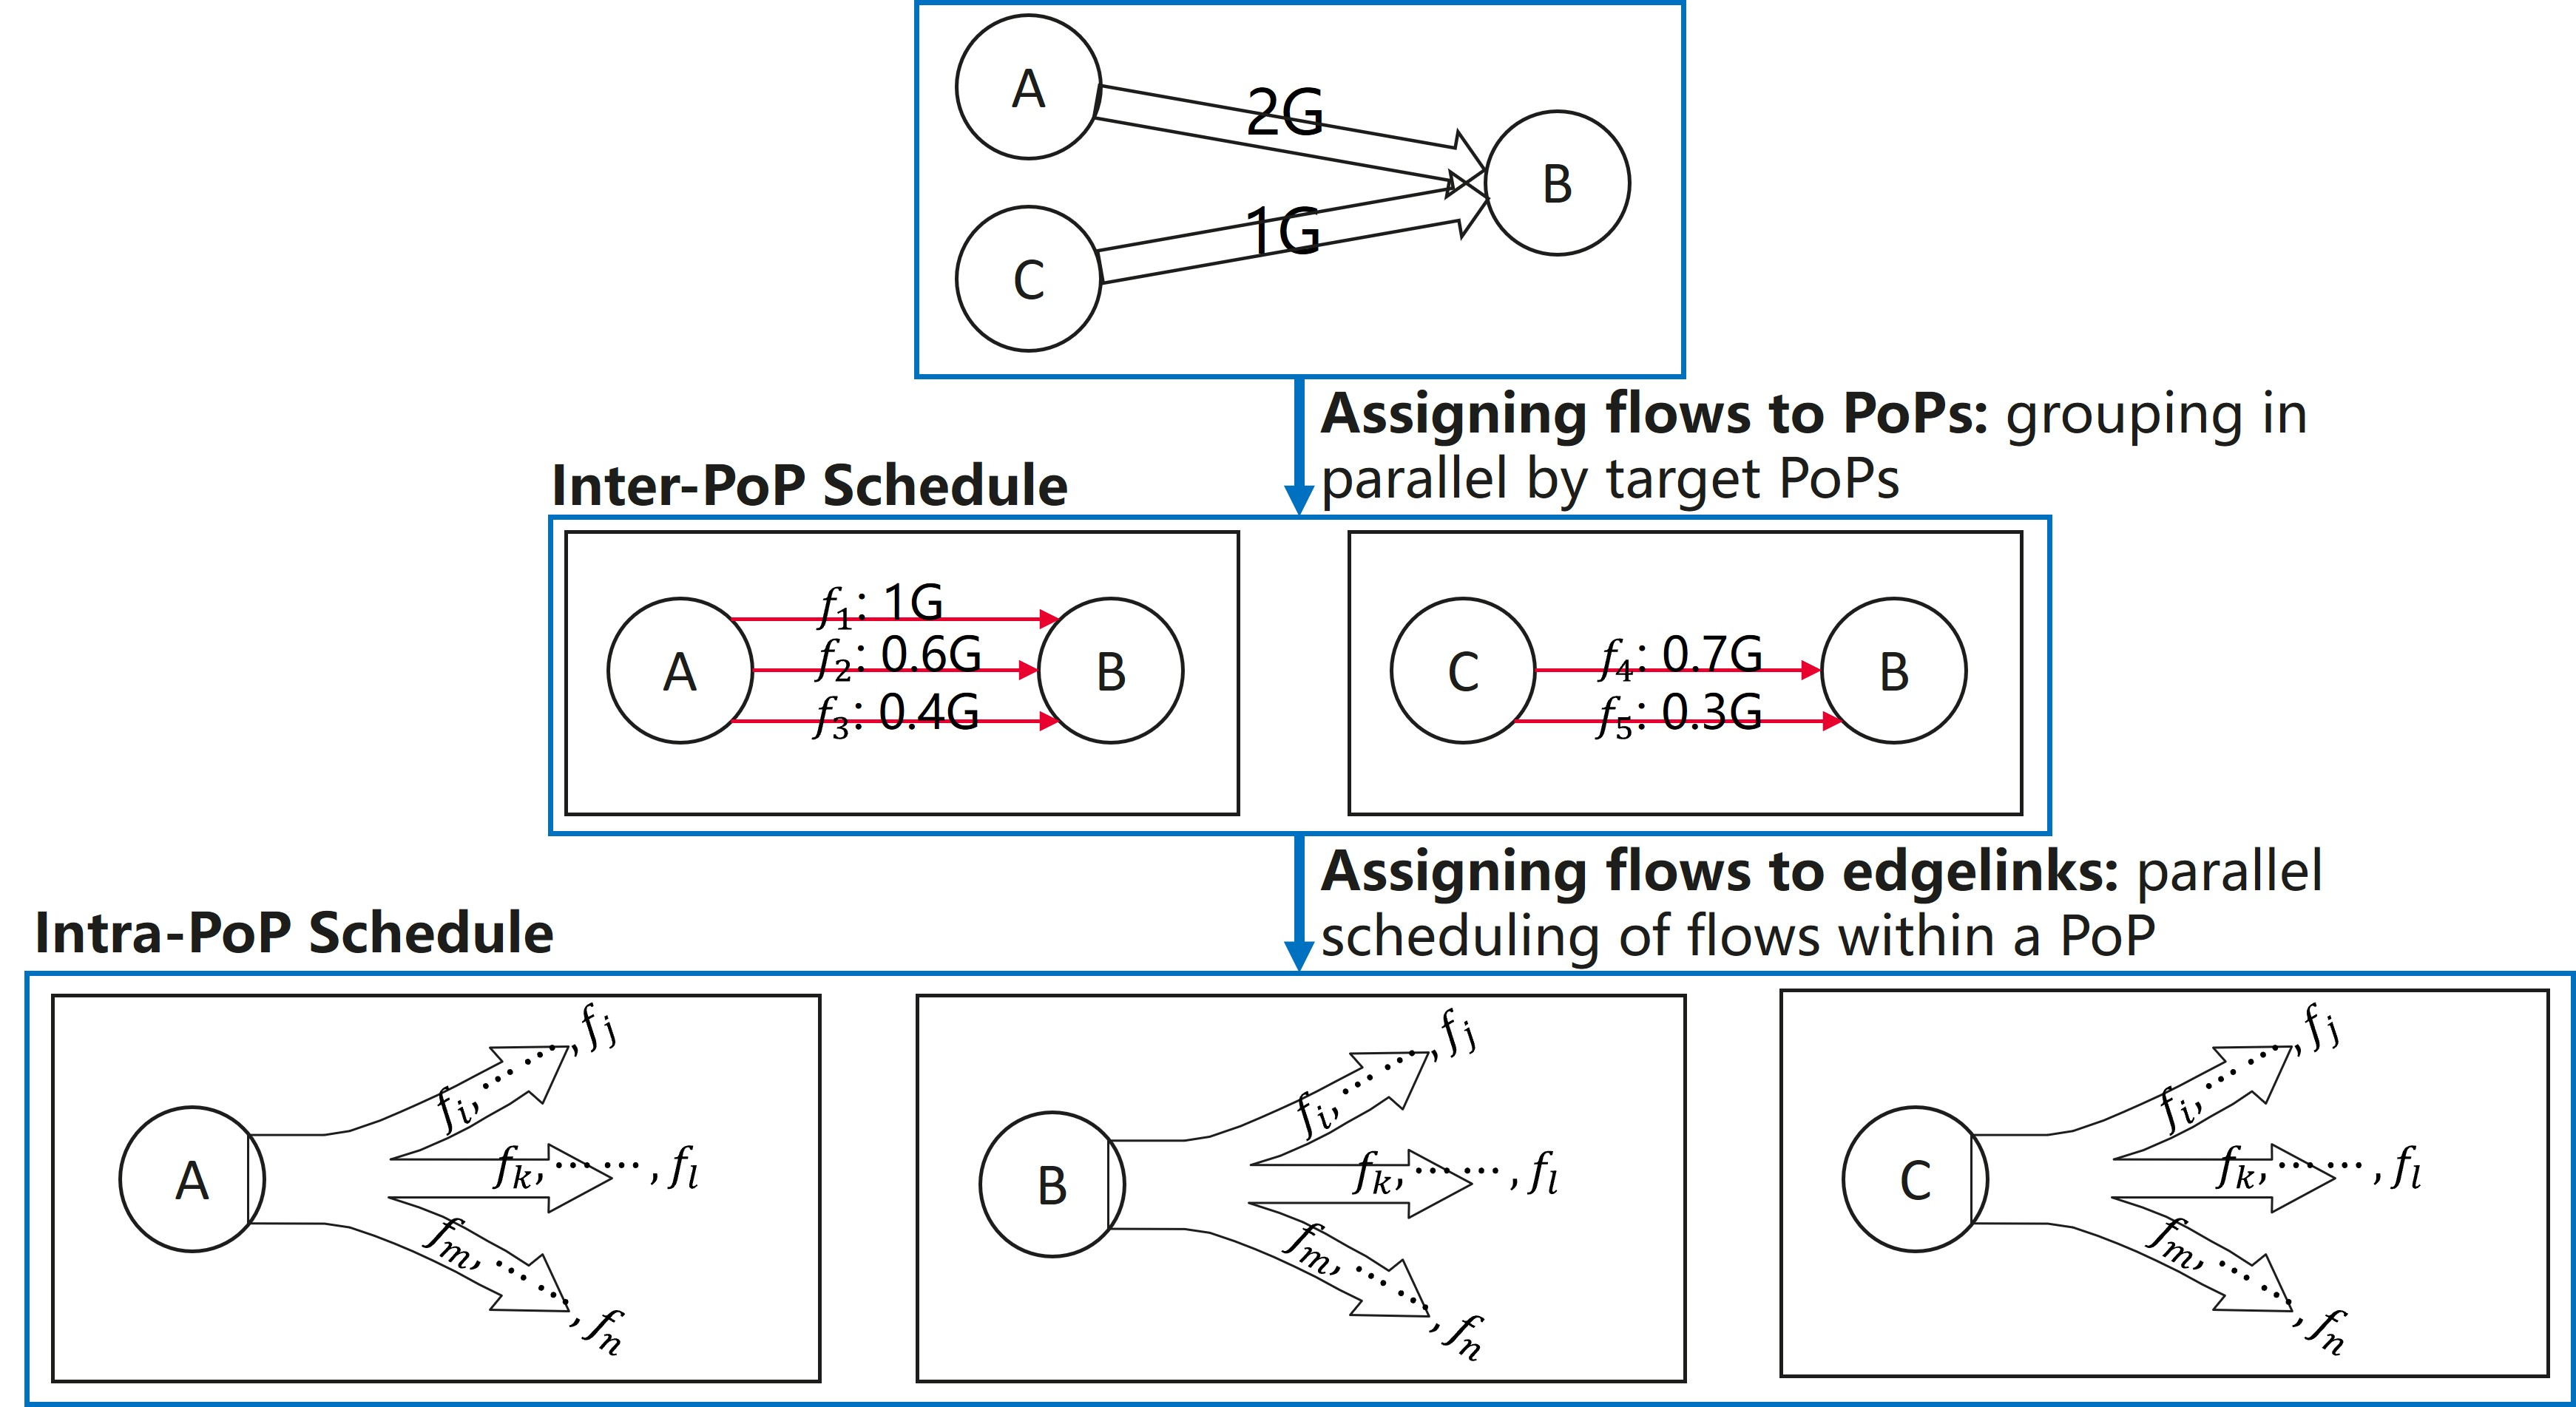
\includegraphics[width = 8cm]{figs/implement/network slicing.jpg}
	\caption{\small An example of slicewise parallelization}
	\label{fig:network slicing}
\end{figure}

% We would like to be able to take parallel operations in all the places that can be parallelized in the above time slot level modules.

% \para{Stream Filtering}
% Filtering of streams will be pulled and filtered in different PoPs in the real present network, which is itself a parallel process, and hence filtering of streams does not need to be parallelized.

% \para{Decision making for {\egress} burst}
% The egress topping decision and the output of the recommended bandwidth for the recommended backbone network is the input of bandwidth data to the solver for computation. The process itself depends only on the value of the bandwidth and the number of PoPs and egresses, and is highly scalable, requiring only 1s-level computation at current scale, and does not require piecewise parallelization. Also if the slice parallelizes the egress egress topping decision, then it must make the resulting topping recommendation and the recommended bandwidth a suboptimal solution.

% \para{Determining the bandwidth size for inter-PoP scheduling}
% Input the topology of the entire network and the recommended bandwidth to pass on the backbone link calculated in step 2, thus outputting the capacity of the virtual backbone link for one hop between each PoP. The time complexity of the algorithm is expected to be $O(n^2 m log(\max{O_u}))$, where n denotes the number of PoPs and m denotes the number of physical backbone links. And since the algorithm is not related to the specific flow but only related to the bandwidth, it has good scalability and does not need to be parallelized.

\para{Slicewise parallel scheduling.}
Slicewise parallel scheduling consists of two steps: inter-PoP scheduling and intra-PoP scheduling. Figure \ref{fig:network slicing} gives an example of slicewise parallelization. After getting the bandwidth of the virtual links between PoPs, the initial step is to conduct inter-PoP scheduling to ensure optimal utilization of the capacity across all virtual links. The process can be easily parallelized efficiently. We assign a thread to each PoP for scheduling flows from that PoP to other PoPs to fill the capacity of the virtual link. In this step, we only schedule non-performance-aware flows into other PoPs without specifying specific {\egress}. Subsequently, each PoP schedules the current flow within its domain to the suitable {\egress}, utilizing the heuristic scheduling strategy outlined in Section \ref{Solving Optimization Quickly}. To enhance the efficiency of the scheduling algorithm, multiple threads can be designated to each PoP for concurrent scheduling.

\para{Network slicing.}
Inspired by the above parallelization method, we propose a simple and efficient network slicing model. One option is that we divide each PoP into a slice, the controllers within each slice run our algorithms individually, and there exists a master controller to issue commands. Initially, controllers within each PoP independently calculate the total traffic within their respective domains and then upload these results to the master controller. The master controller makes the {\egress} burst decision and allocates the virtual link capacity between PoPs. Subsequently, the master controller communicates the virtual link capacity to the controllers within each PoP. Lastly, controllers within each PoP finalize the flow scheduling using a process akin to the parallel algorithm. The described slicing scheme offers the advantage of being straightforward, efficient, and easily implementable without causing undue inter-controller message transmission overheads. Since the capacity of the backbone is very limited and the algorithm greedily fills the virtual link capacity with large flows, the number of flows scheduled between PoPs will not be very large (typically less than 20,000 in tests). Moreover, for specific scenarios where it is desirable to incorporate multiple PoPs as a single slice, the slice scheme outlined above can be conveniently adjusted.
% Heuristic scheduling flows are categorized into: scheduling performance-aware flows, scheduling cost flows.

% \begin{itemize}[leftmargin=*] 
% \item
% Scheduling performance-aware flows needs to probe all the feasible {\egresses} it corresponds to and then pick the lowest delay egress and assign it. This step uses inter-PoP parallelism. A thread is allocated in each PoP to go to the performance-aware queue and take out a performance-aware flow and assign it to the egress with the lowest delay among its feasible egresses, locking the egresses being traversed in the meantime.
% \item Scheduling Non-performance-aware Flows
% Scheduling a cost flow is a two-step process: Step 1, select the cost flows within the PoP that need to be scheduled across PoPs and assign them to the target PoP. Step 2, assign all the flows to be dispatched within the PoP. Step 1 is naturally inter-PoP parallelism, where a thread in each PoP is assigned to pick which streams need to be scheduled across PoPs and assign those streams that need to be scheduled across PoPs to the Incoming queue of the target PoP. Step 2 is to assign the streams in the Incoming queue and the streams that are still remaining after cross-PoP scheduling to the egress of the PoP. We observe that the size of the flows on different PoPs varies very much, and the flows in the PoPs are unevenly distributed, with very large flows in Singapore and Hong Kong. If we allocate only one thread within a PoP, performing parallel acceleration between PoPs has limited effect. Therefore, we choose to perform intra-PoP parallelism in this step. We assign a corresponding number of threads to the PoP in proportion to the PoP's stream size (based on the total number of threads that can be used), and then each thread goes to the Incoming queue and the default stream's pending queue to get the streams, assigns them to the egresses whose bandwidths are not up to the available capacity among the egresses in the PoP, and locks the egresses while checking whether it can be assigned to a particular egress.
% \end{itemize}

% \para{Increase $p_i$}
% The process is to assign a flow to the egress with the least increase in egress cost for all remaining flows. Therefore we directly allocate a certain number of threads to go and pick up the streams in order from the remaining stream queue, and then implement parallelism by putting a lock on an egress while traversing it.


\subsection{Routing Table Compression}
{\sys} uses compact data structures and efficient algorithms (\S \ref{sec:scheduling}) to flexibly forward traffic. The following problem is large scale ipv4, ipv6 routes. {\sys} was responsible for routing datacenter prefixes only, which were few enough for all SWAN routers to run BGP and store the datacenter routing tables in the router memory. {\sys} routers had to contend with Internet routing tables and it would be cost prohibitive to make every {\sys} router hold the entire Internet routing table.  Each entry in the raw routing table consists of a prefix and a series of routing information (e.g., next hop, origin, as path, and etc.), so a single 64GB router can store about only 15 million raw routing entries. Hence, {\sys} assigned two roles to routers: (1) aggregation routers that hold full IP routing tables, and (2) backbone routers that act as forwarding only nodes that do not run BGP. We develop a new SDN function in {\sys} called traffic steering on aggregation routers to encapsulate WAN packets with information needed by backbone routers to do TE without IP routing. 

\iffalse
\begin{figure}
\centering
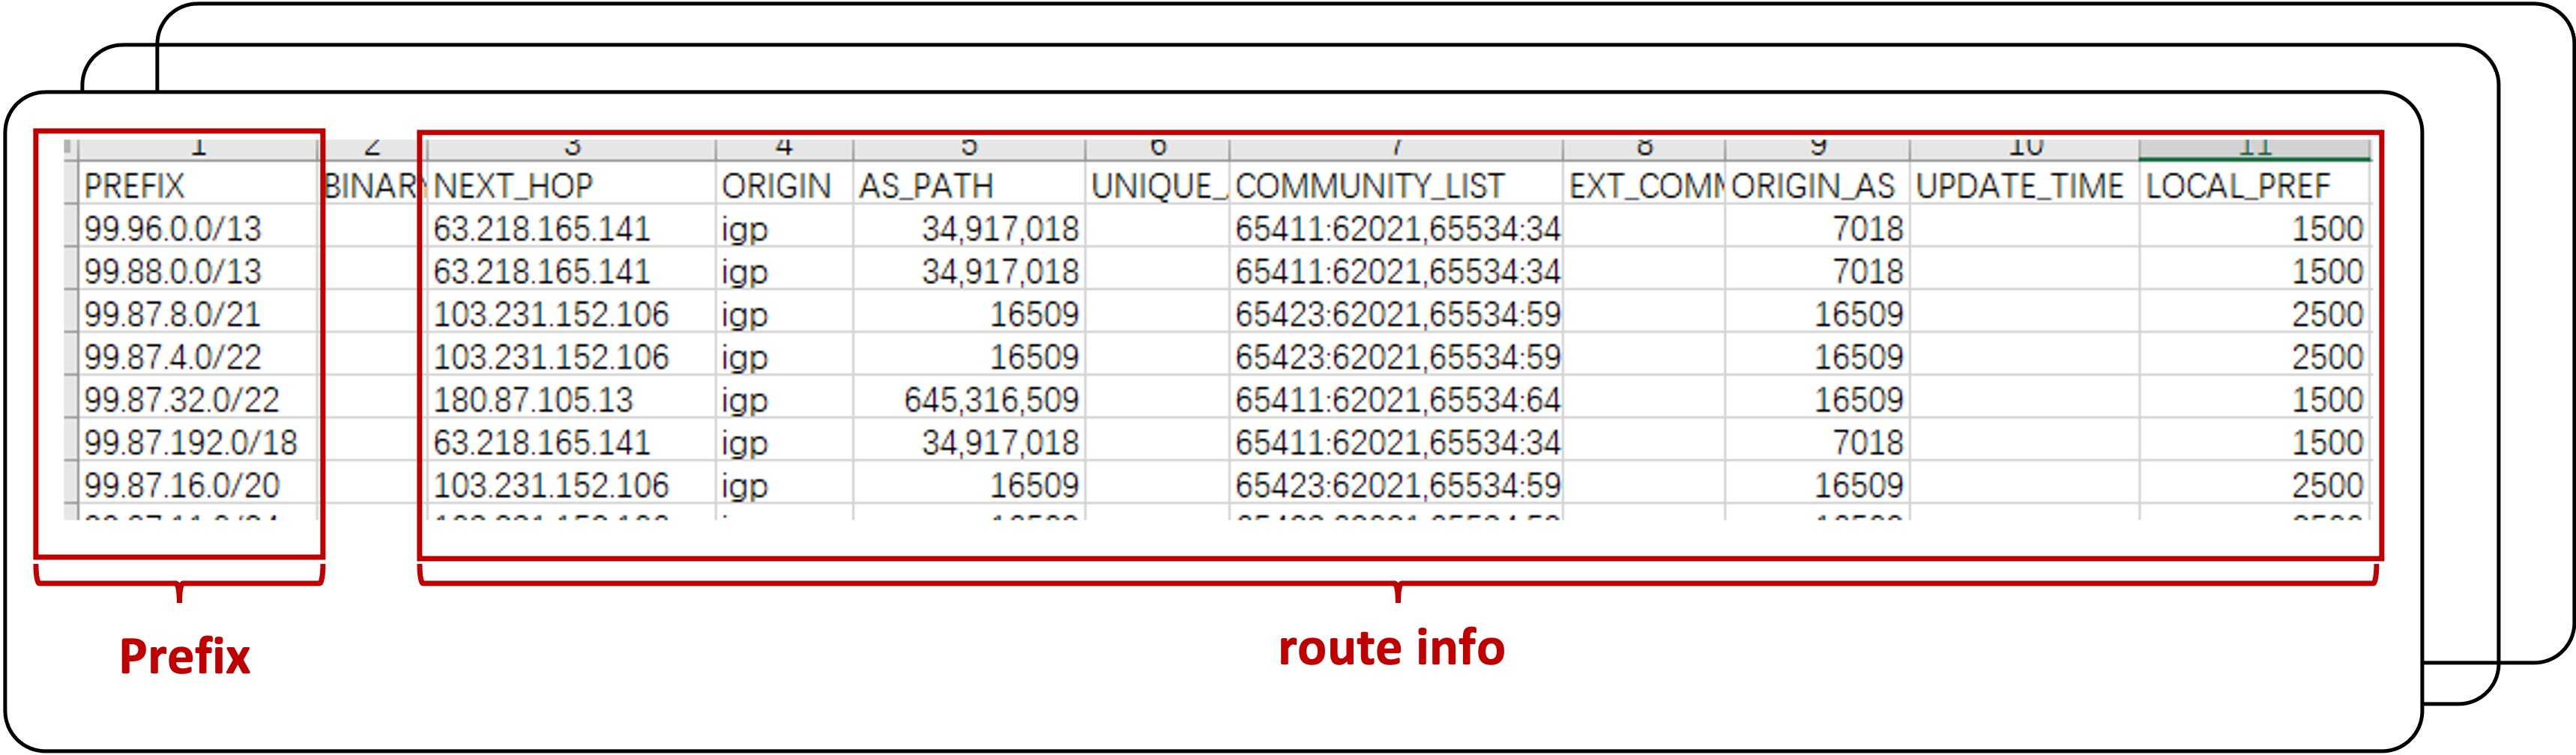
\includegraphics[width = 8cm]{figs/routetable.jpg}
\caption{\small Routing Information Database (RIB)}
\label{fig:routetable}
\end{figure}
\fi

\iffalse
\begin{figure}
\centering
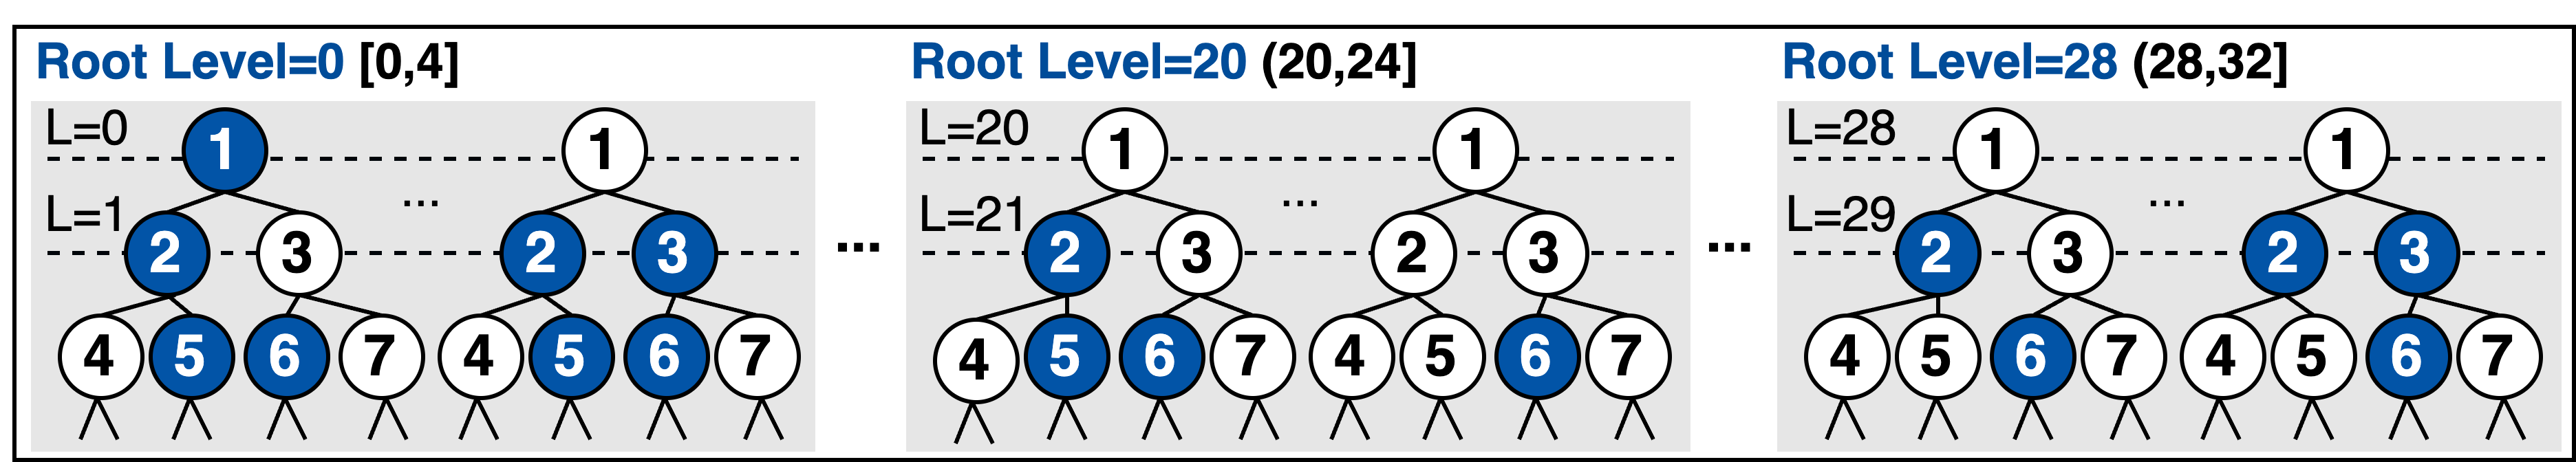
\includegraphics[width = 8cm]{figs/nsdi-forest.png}
\caption{\small Logical and Memory Data Structure: Forest}
\label{fig:treestructure}
\end{figure}
\fi

\begin{figure}
\centering
\subfigure[Logical structure]{
	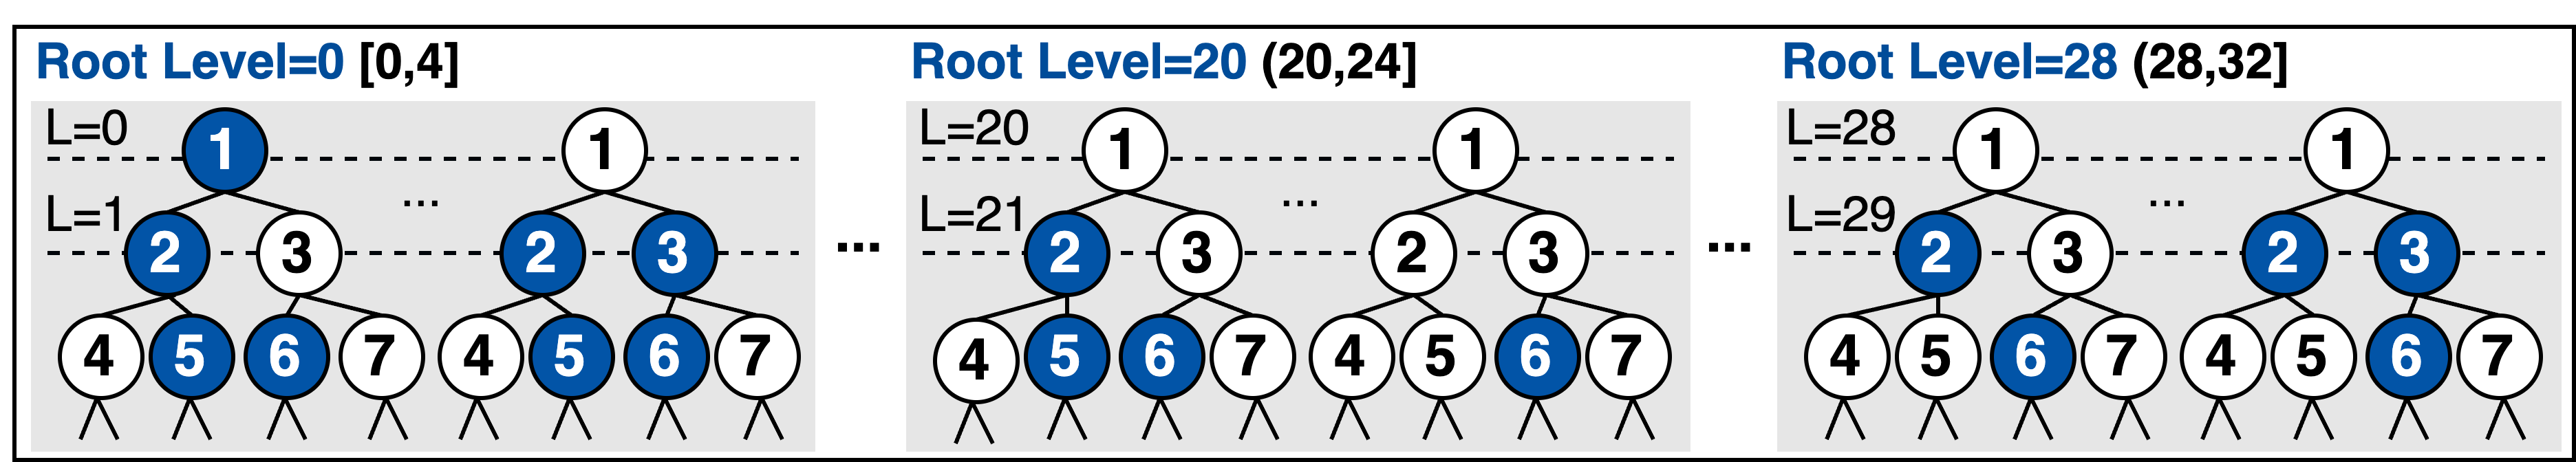
\includegraphics[width=\linewidth]{figs/nsdi-forest.png}}
\label{fig:forest-logical}
%\quad
\subfigure[Memory structure]{
	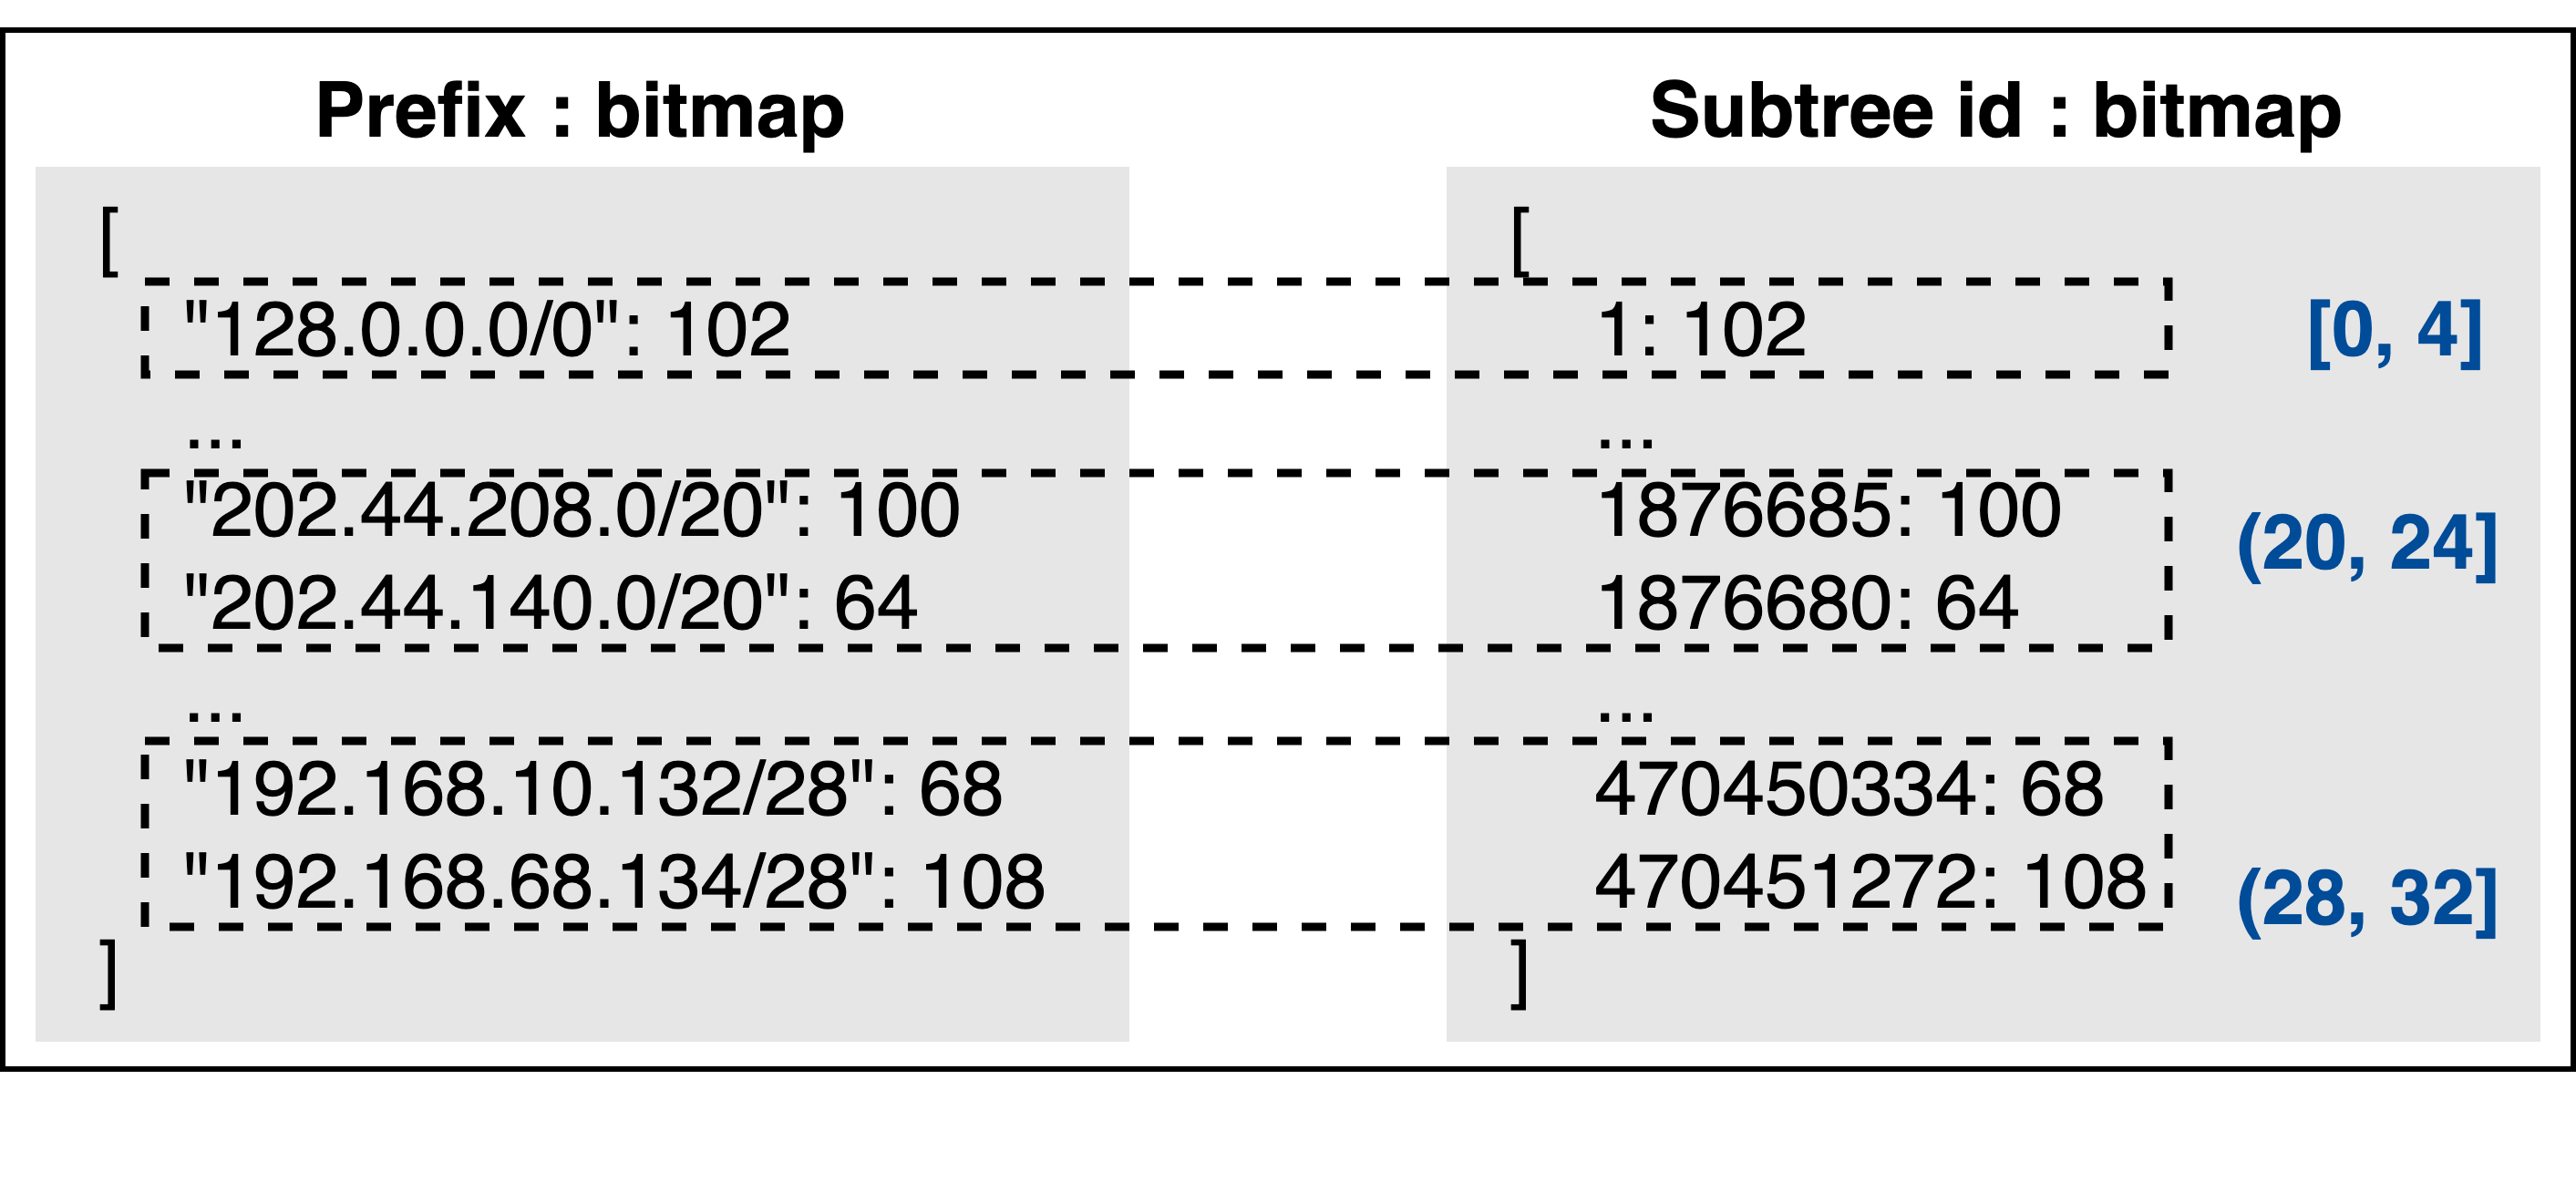
\includegraphics[width=\linewidth]{figs/nsdi-forest-mem.png}}\label{fig:forest-mem}
\caption{\small Logical and Memory Data Structure: Forest}
\label{fig:foreststructure}
\end{figure}


%As illustrated in Figure \ref{fig:routetable}, 
%Generally, each entry in the raw routing table consists of a prefix and a series of routing information (e.g., next hop, origin, as path, and etc.). 
Currently, some tree-based index structures are used to compress the raw routing table, such as Binary tree\cite{binarytree}, Patricia trie\cite{szpankowski1990patricia}, Radix tree\cite{sklower1991tree}, TreeBitmap\cite{eatherton2004tree}, Poptrie\cite{asai2015poptrie}, and etc. However, the memory of a single {\sys} controller cannot afford the whole compressed index of routing table entries for the entire network, making routing computations require a large number of data exchanges between memory and storage, , e.g., longest matching, full matching, subnet matching, field filtering, and etc. In other words, compressing all routes into one tree will cause the depth of the tree to be too large, which will affect routing index construction and calculation efficiency. Moreover, frequent updates on a large tree also incurs a large computation overhead. Therefore, we need to consider how to efficiently  compress routing entry indexes and ensure the  functions and performance of dynamic addition, deletion, modification, and query.

%{binarytree}: Waldvogel, Marcel, et al. "Scalable high speed IP routing lookups." Proceedings of the ACM SIGCOMM'97 Conference on Applications, technologies, architectures, and protocols for computer communication. 1997.

%{Patricia trie}: Szpankowski, W., "Patricia tries again revisited," Journal of the Association for Computing Machinery, vol.37, no.4, p. 691-711.

%{radixtree}: Routing on longest-matching prefixes

%{radixtree}: Keith Sklower, A Tree-Based Packet Routing Table for Berkeley Unix, USENIX Winter 1991: 93-104.

%{treebitmap}: Eatherton, Will, George Varghese, and Zubin Dittia. "Tree bitmap: hardware/software IP lookups with incremental updates." ACM SIGCOMM Computer Communication Review 34.2 (2004): 97-122.

%{Poptrie}: Asai, Hirochika, and Yasuhiro Ohara. "Poptrie: A compressed trie with population count for fast and scalable software IP routing table lookup." ACM SIGCOMM Computer Communication Review 45.4 (2015): 57-70.

In order to improve efficiency, we need to control the scope of route calculation and update as locally as possible. Therefore, we propose a hierarchical forest-based index structure, as illustrated in Fig. \ref{fig:forest-logical}, which decomposes a large tree into multiple flattened subtrees according to the prefix hierarchy, (e.g., $[/16, /20], [/20, /24]$), so that not only the path length of route calculation can be reduced, but also the scope of routing update can be controlled in a small subtree. 

However, the space overhead of maintaining the hierarchical forest directly in memory is still non-trivial. We further propose a more compact routing index structure, \emph{ForestBitmap}, to compress each subtree, and the memory overhead can be greatly reduced by mapping each subtree to an entry in memory that is uniquely represented by two integers, i.e., subtree id and the bitmap, as illustrated in Fig. \ref{fig:forest-mem}. In addition, routing computations are mainly implemented by bit operations with high efficiency and routing queries do not need to performed on the tree to avoid deep search and backtracking of excessive trails. This compact and flexible index structure can achieve $O(1)$ online update performance and is easy to expand.

\begin{figure}
	\centering
	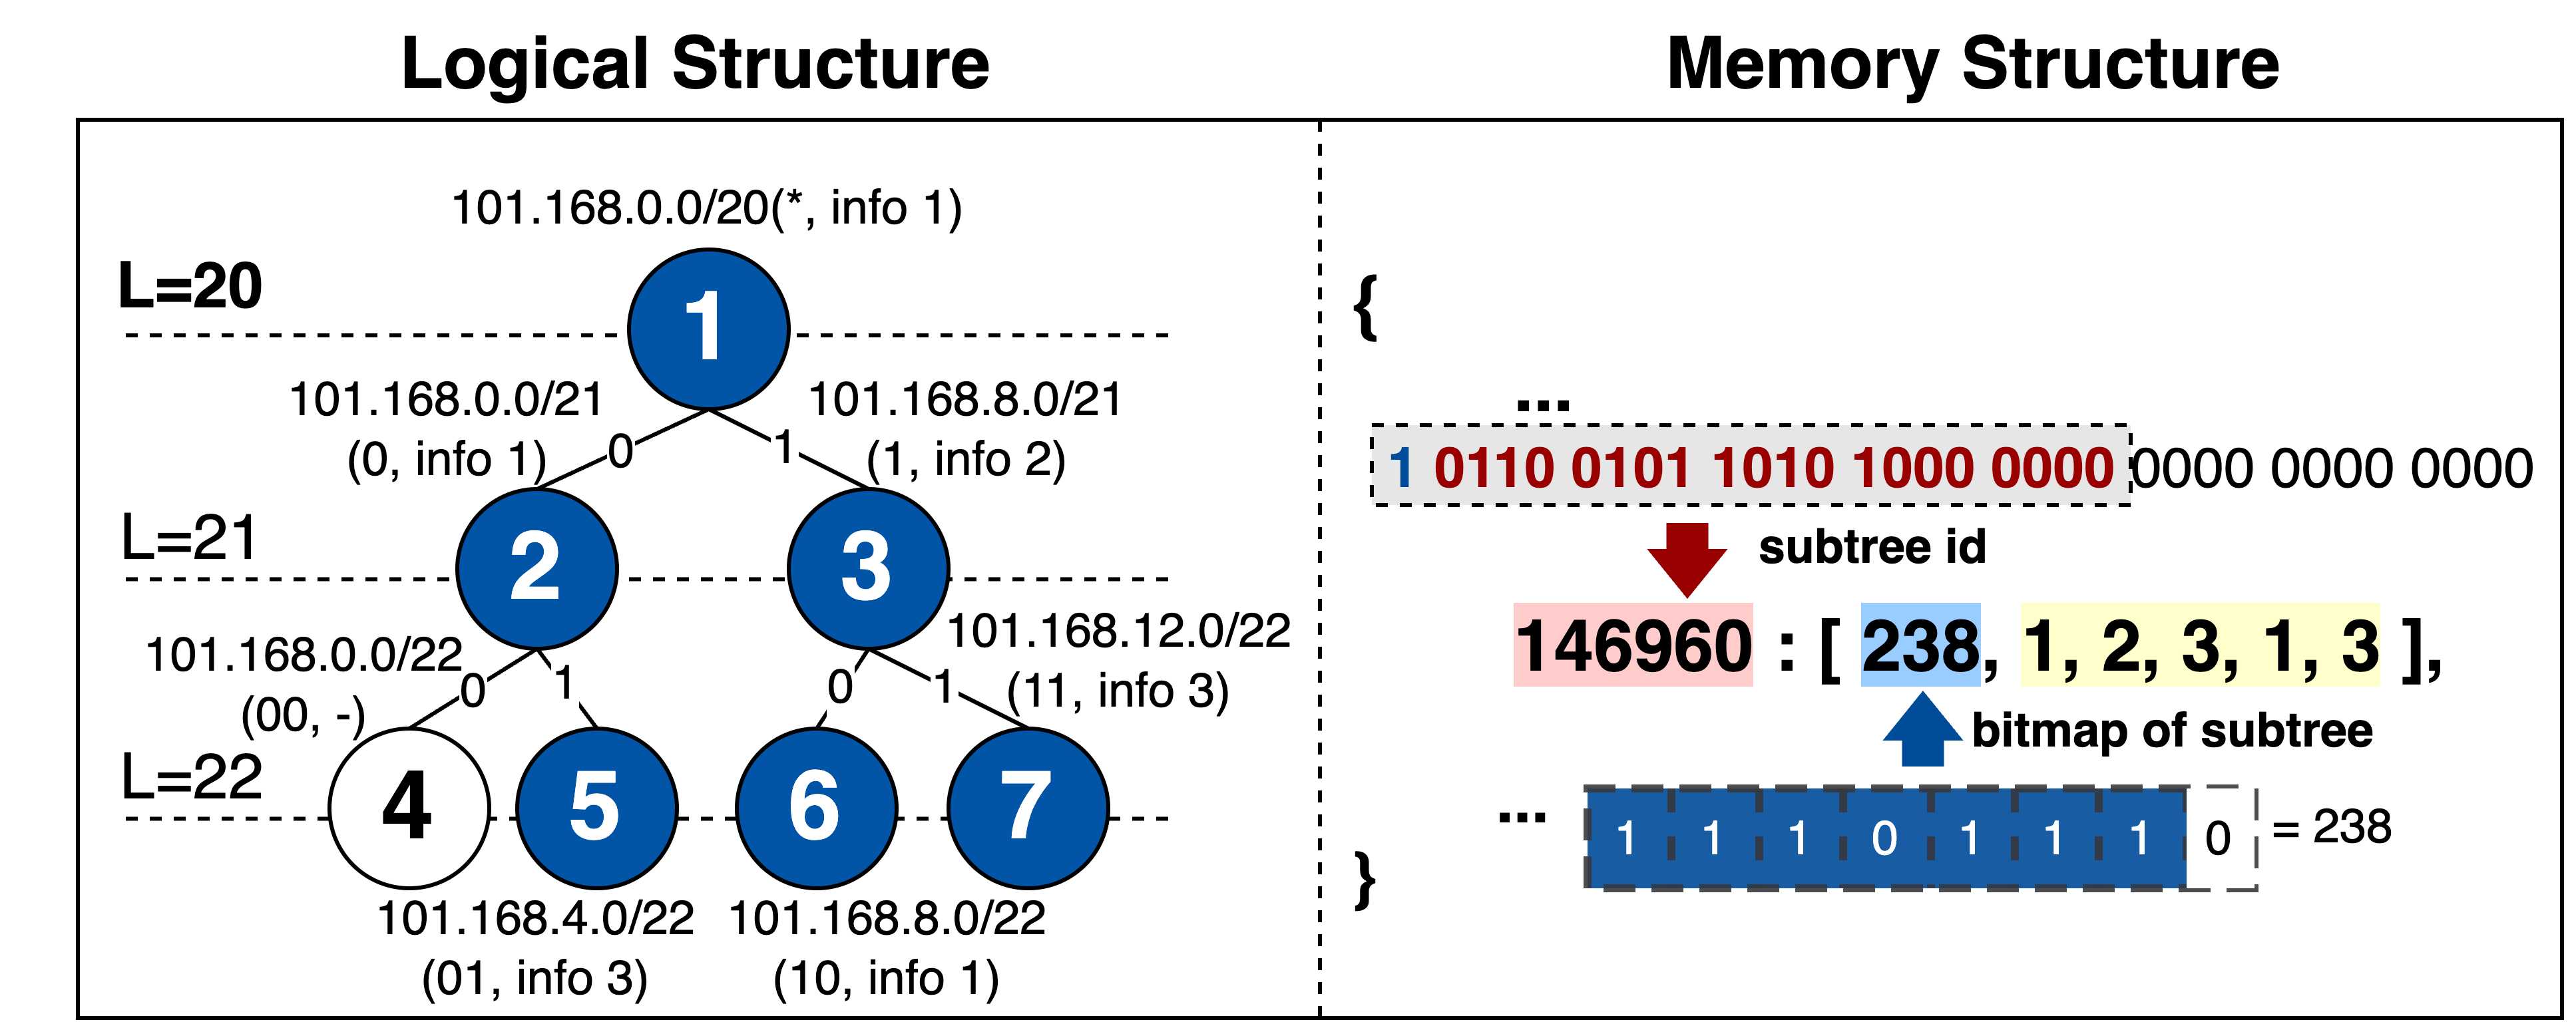
\includegraphics[width=\linewidth]{figs/nsdi-tree.png}
	\caption{\small Logical and Memory Data Structure: Subtree}
	\label{fig:treestructure}
\end{figure}


More specifically, we take the 3-layer subtree in Fig. \ref{fig:treestructure} as an example to illustrate the subtree compression encoding process. Subtree index id is calculated based on the common binary prefix through subnet aggregation, i.e, 0110 0101 1010 1000 0000, and padded the most significant bit with 1 to get the unique subtree id 1464960. Based on the subtree id, we can uniquely locate the subtree where the route resides.  
Since a 3-layer subtree can store up to seven routes, we use 8-bit bitmap to encode non-null nodes and obtain 238 (i.e., 11101110), where the least significant bit is a reserved bit. Regardless of the pure prefix index, we should consider the more general case of storing and indexing the whole routing tables with attribute information. \emph{ForestBitmap} encodes  the route attribute information  lexicographically and shares them among all routes, whose id is inserted after bitmap based on the sequence of valid bits accordingly. So far, we can compress a 3-layer subtree that contains routing table entries into a Map entry in memory, where the key is the subtree id and the value is an array that contains bitmap and a series of attribute information id(s). 

\emph{Remark.} Taking IPv4 as an example, a 5-layer subtree that stores 31 routing table entries can be represented by a Map entry, so that the IPv4 BGP routing entries with more than 900,000 unique prefixes can be compressed to less than 170,000 Map entries. Compared with the simple tree structures, the memory compression ratio is higher, because of the  compact data structures and aligned integer encoding, and it is more suitable to be placed in the cache to improve the hit rate.

\begin{table}[tbp]
	%	\footnotesize
	\centering
	\resizebox{0.48\textwidth}{7mm}{
		\begin{tabular}{c|c|c}
			\hline
			Memory (MB) & Prefix Index & Routing Index  \\ 
			\hline
			Baseline (Google RadixTree\cite{googleradixtree}) & 204.37 &	556.48 \\ 
			\hline
			{\sys}& 11.55 & 95.31   \\ 
			\hline
			Optimization &  17.69$\times$ & 5.93$\times$ \\ 
			\hline
		\end{tabular}
	}
	\vspace{-0.1in}
	\caption{\small Memory optimization of \emph{ForestBitmap}}
	\label{tab:compression-mem}
\end{table}

% Google Radix Tree: https://code.google.com/archive/p/radixtree/

\begin{table}[tbp]
	%	\footnotesize
	\centering
	\resizebox{0.48\textwidth}{7mm}{
		\begin{tabular}{c|c|c|c|c|c|c|c}
			\hline
			Time (ms) & Index Build & Longest Match & Full Match & Subnet  Match & Delete & Origin\_as Filter & Update  \\ 
			\hline
			Baseline (Google RadixTree\cite{googleradixtree}) & 1534 &	4.463 & 8.251 & 758.3 & 122.6 & 75.44 & 1306 \\ 
			\hline
			{\sys}& 533.8 & 1.453 & 2.554 & 39.31 & 25.76 & 55.79 & 81.31 \\ 
			\hline
			Optimization & 2.87$\times$ & 3.07$\times$ & 3.23$\times$ & 19.29$\times$ & 4.75$\times$ & 1.35$\times$ & 16.06$\times$ \\ 
			\hline
		\end{tabular}
	}
	\vspace{-0.1in}
	\caption{\small Routing computation optimization of \emph{ForestBitmap}}
	\label{tab:compression-time}
\end{table}

The results on live network data set show that our \emph{ForestBitmap} achieves a compression ratio of 17.69x compared with the baseline for pure prefix index in Table \ref{tab:compression-mem}. For the complete routing index, \emph{ForestBitmap} achieves a compression ratio of 5.83 times in Table \ref{tab:compression-mem} and a computing efficiency improvement of 1.35 times to 19.29 times in Table \ref{tab:compression-time}.


\iffalse
%As illustrated in Figure \ref{fig:routetable}, 
Generally, each entry in the raw routing table consists of a prefix and a series of routing information (e.g., next hop, origin, as path, and etc.). If the raw routing table is stored and indexed directly in memory, the memory overhead and computational efficiency are very low. Moreover, the current popular index structures based on the radix tree, such as  can not be completely stored in the {\sys} controller. In order to efficiently index and maintain routing tables in the memory, we propose a more compact data structure, \emph{ForestBitmap}, to store routing table and ensure routing computation. (e.g., longest matching, full matching, subnet matching, field filtering, and dynamic route addition, deletion, and modification, etc.)


\todo{Hierarchical Forest based Online Routing Index:}
First, we divide the routing prefix to get some partitions (e.g., $[/16, /20], [/20, /24]$), and make them cover the entire IP prefix range. Then, we consider to aggregate prefixes and compress routing entries with common binary prefixes into a logical subtree, based on the observed strict hierarchical relationship among the prefixes. As shown in Figure \ref{fig:treestructure}, a logical storage structure of a three-layer subtree on the left is obtained by aggregating six routes with three kinds of attributes information according to their prefixes. After that, we map the logical subtree into memory using a more compact data structure to reduce the memory occupied by routing entries.

\todo{Subtree compression: aligned integer encoding}
More specifically, We truncate the common binary part of them, i.e, 0110 0101 1010 1000 0000, and padded the most significant bit with 1 to get the unique subtree id 1464960. Based on the subtree id, we can uniquely determine the subtree where the route is located. Since a three-layer subtree can store up to seven routes, we use 8-bit bitmap to encode non-null nodes and obtain 238 (i.e., 11101110), where the least significant bit is a reserved bit. In addition, the route attribute information is lexicographically encoded, whose id is inserted after bitmap based on the sequence of valid bits accordingly. So far, we compress a three-layer subtree that contains routing table entries into a Map entry in memory, where the key is the subtree id and the value is an array that contains bitmap and a series of attribute information id(s). Note that in the case of IPv4, if we set the layers of subtree to 5, we can represent 31 routes per Map entry. So, for IPv4 BGP routing entries with 918773 unique prefixes, this compact structure requires only 163794 Map entries.
\fi